\documentclass[11pt,a4paper]{article}
\usepackage[utf8]{inputenc}
\usepackage{amsmath, amsthm, amssymb}
\usepackage[table]{xcolor}
\usepackage{graphicx}
\usepackage{hyperref}
\usepackage[a4paper, left=0.5in, right=0.5in, top=1in, bottom=1in]{geometry}
\documentclass{article}

\usepackage[fontsize=13pt]{scrextend}
\usepackage{multicol}
\usepackage{lmodern} % For scalable Computer Modern fonts % Ensures proper font encoding
\usepackage{color}
\usepackage{helvet}  % For changing fonts

\usepackage{soul}  % For highlighting

\geometry{
  a4paper,
  left=25mm,
  right=25mm,
  top=25mm,
  bottom=25mm,
  heightrounded,
}
% Required packages
\usepackage{tikz}
\usepackage{enumitem}
\usepackage{booktabs}
\usepackage{tabularx}
\usepackage[many]{tcolorbox}
\usepackage{mdframed}

% Custom styling
\newcommand{\subsecformat}[1]{%
    \vspace{0.5em}
    \noindent\tikz\draw[line width=0.4pt] (0,0) -- (\textwidth,0);
    \vspace{-1.5em}
    \subsection*{\textsf{#1}}
    \vspace{-0.5em}
}

% Define a custom frame style
\mdfdefinestyle{mythick}{%
    linewidth=0.4pt,
    leftline=false,
    rightline=false,
    innerleftmargin=0pt,
    innerrightmargin=0pt,
    innertopmargin=4pt,
    innerbottommargin=4pt
}

% Custom list style
\newenvironment{compactlist}{%
    \begin{itemize}[leftmargin=*,itemsep=0.2em,parsep=0pt,topsep=0pt]
}{\end{itemize}}


\usepackage{lastpage} % Required to determine the last page number for the footer

\usepackage{graphicx} % Required to insert images

\setlength\parindent{0pt} % Removes all indentation from paragraphs

\usepackage[most]{tcolorbox} % Required for boxes that split across pages

\usepackage{booktabs} % Required for better horizontal rules in tables

\usepackage{listings} % Required for insertion of code

\usepackage{etoolbox} % Required for if statements

%----------------------------------------------------------------------------------------
%	MARGINS
%----------------------------------------------------------------------------------------

\usepackage{geometry} % Required for adjusting page dimensions and margins

\geometry{
	paper=a4paper, % Change to letterpaper for US letter
	top=3cm, % Top margin
	bottom=3cm, % Bottom margin
	left=2.5cm, % Left margin
	right=2.5cm, % Right margin
	headheight=14pt, % Header height
	footskip=1.4cm, % Space from the bottom margin to the baseline of the footer
	headsep=1.2cm, % Space from the top margin to the baseline of the header
	%showframe, % Uncomment to show how the type block is set on the page
}

%----------------------------------------------------------------------------------------
%	FONT
%----------------------------------------------------------------------------------------

\usepackage[utf8]{inputenc} % Required for inputting international characters
\usepackage[T1]{fontenc} % Output font encoding for international characters

\usepackage[sfdefault,light]{roboto} % Use the Roboto font

%----------------------------------------------------------------------------------------
%	HEADERS AND FOOTERS
%----------------------------------------------------------------------------------------

\usepackage{fancyhdr} % Required for customising headers and footers

\pagestyle{fancy} % Enable custom headers and footers

\lhead{\small\assignmentClass\ifdef{\assignmentClassInstructor}{\ (\assignmentClassInstructor):}{}\ \assignmentTitle} % Left header; output the instructor in brackets if one was set
\chead{} % Centre header
\rhead{\small\ifdef{\assignmentAuthorName}{\assignmentAuthorName}{\ifdef{\assignmentDueDate}{Due\ \assignmentDueDate}{}}} % Right header; output the author name if one was set, otherwise the due date if that was set

\lfoot{} % Left footer
\cfoot{\small Page\ \thepage\ of\ \pageref{LastPage}} % Centre footer
\rfoot{} % Right footer

\renewcommand\headrulewidth{0.5pt} % Thickness of the header rule

%----------------------------------------------------------------------------------------
%	MODIFY SECTION STYLES
%----------------------------------------------------------------------------------------

\usepackage{titlesec} % Required for modifying sections
\usepackage{longtable}
\documentclass{article}
%------------------------------------------------
% Section

\titleformat
{\section} % Section type being modified
[block] % Shape type, can be: hang, block, display, runin, leftmargin, rightmargin, drop, wrap, frame
{\Large\bfseries} % Format of the whole section
{\assignmentQuestionName~\thesection} % Format of the section label
{6pt} % Space between the title and label
{} % Code before the label

\titlespacing{\section}{0pt}{0.5\baselineskip}{0.5\baselineskip} % Spacing around section titles, the order is: left, before and after

%------------------------------------------------
% Subsection

\titleformat
{\subsection} % Section type being modified
[block] % Shape type, can be: hang, block, display, runin, leftmargin, rightmargin, drop, wrap, frame
{\itshape} % Format of the whole section
{(\alph{subsection})} % Format of the section label
{4pt} % Space between the title and label
{} % Code before the label

\titlespacing{\subsection}{0pt}{0.5\baselineskip}{0.5\baselineskip} % Spacing around section titles, the order is: left, before and after

\renewcommand\thesubsection{(\alph{subsection})}

%----------------------------------------------------------------------------------------
%	CUSTOM QUESTION COMMANDS/ENVIRONMENTS
%----------------------------------------------------------------------------------------

% Environment to be used for each question in the assignment
\newenvironment{question}{
	\vspace{0.5\baselineskip} % Whitespace before the question
	\section{} % Blank section title (e.g. just Question 2)
	\lfoot{\small\itshape\assignmentQuestionName~\thesection~continued on next page\ldots} % Set the left footer to state the question continues on the next page, this is reset to nothing if it doesn't (below)
}{
	\lfoot{} % Reset the left footer to nothing if the current question does not continue on the next page
}

%------------------------------------------------

% Environment for subquestions, takes 1 argument - the name of the section
\newenvironment{subquestion}[1]{
	\subsection{#1}
}{
}

%------------------------------------------------

% Command to print a question sentence
\newcommand{\questiontext}[1]{
	\textbf{#1}
	\vspace{0.5\baselineskip} % Whitespace afterwards
}

%------------------------------------------------

% Command to print a box that breaks across pages with the question answer
\newcommand{\answer}[1]{
	\begin{tcolorbox}[breakable, enhanced]
		#1
	\end{tcolorbox}
}

%------------------------------------------------

% Command to print a box that breaks across pages with the space for a student to answer
\newcommand{\answerbox}[1]{
	\begin{tcolorbox}[breakable, enhanced]
		\vphantom{L}\vspace{\numexpr #1-1\relax\baselineskip} % \vphantom{L} to provide a typesetting strut with a height for the line, \numexpr to subtract user input by 1 to make it 0-based as this command is
	\end{tcolorbox}
}

%------------------------------------------------

% Command to print an assignment section title to split an assignment into major parts
\newcommand{\assignmentSection}[1]{
	{
		\centering % Centre the section title
		\vspace{2\baselineskip} % Whitespace before the entire section title
		
		\rule{0.8\textwidth}{0.5pt} % Horizontal rule
		
		\vspace{0.75\baselineskip} % Whitespace before the section title
		{\LARGE \MakeUppercase{#1}} % Section title, forced to be uppercase
		
		\rule{0.8\textwidth}{0.5pt} % Horizontal rule
		
		\vspace{\baselineskip} % Whitespace after the entire section title
	}
}

%----------------------------------------------------------------------------------------
%	TITLE PAGE
%----------------------------------------------------------------------------------------

\author{\textbf{\assignmentAuthorName}} % Set the default title page author field
\date{} % Don't use the default title page date field

\title{
	\thispagestyle{empty} % Suppress headers and footers
	\vspace{0.2\textheight} % Whitespace before the title
	\textbf{\assignmentClass:\ \assignmentTitle}\\[-4pt]
	\ifdef{\assignmentDueDate}{{\small Due\ on\ \assignmentDueDate}\\}{} % If a due date is supplied, output it
	\ifdef{\assignmentClassInstructor}{{\large \textit{\assignmentClassInstructor}}}{} % If an instructor is supplied, output it
	\vspace{0.32\textheight} % Whitespace before the author name
}


\usepackage[utf8]{inputenc}
\usepackage[T1]{fontenc}
\usepackage{lmodern}
\usepackage{booktabs}
\usepackage{xcolor}
\usepackage{tikz}
\usepackage{pgfplots}
\usepackage{graphicx}

\usepackage{amsmath}


\usepackage{amsfonts}
\usepackage{amssymb}

\usepackage{tabularx}



\usepackage{hyperref}
\usepackage{listings}
\usepackage{booktabs}
\usepackage{tabularray}
\usepackage{multirow}
\usepackage{float}
\usepackage{lastpage}
\usepackage{tcolorbox}
\usepackage{titlesec}

\usepackage{etoolbox}

\makeatletter
\patchcmd{\@zfancyhead}{\fancy@reset}{\f@nch@reset}{}{}
\patchcmd{\@set@em@up}{\f@ncyolh}{\f@nch@olh}{}{}
\patchcmd{\@set@em@up}{\f@ncyolh}{\f@nch@olh}{}{}
\patchcmd{\@set@em@up}{\f@ncyorh}{\f@nch@orh}{}{}
\makeatother

\pgfplotsset{compat=newest}

% Colors from structure.tex
\definecolor{secondaryColor}{RGB}{0,0,0}
\definecolor{accentColor1}{RGB}{255,87,34}
\definecolor{accentColor3}{RGB}{63,81,181}
\definecolor{textColor}{RGB}{33,33,33}
\definecolor{primaryColor}{RGB}{34, 45, 101}
\definecolor{accentColor2}{RGB}{46, 117, 182}
\definecolor{backgroundColor}{RGB}{245, 245, 245}
\definecolor{fitcolor}{RGB}{0,128,0}
\definecolor{okaycolor}{RGB}{255,165,0}
\definecolor{notfitcolor}{RGB}{255,0,0}

% Define colors
\definecolor{brightred}{RGB}{255,0,0}
\definecolor{brightgreen}{RGB}{0,255,0}
\definecolor{brightblue}{RGB}{0,0,255}
\definecolor{brightyellow}{RGB}{255,255,0}
\definecolor{brightorange}{RGB}{255,165,0}
\definecolor{brightpurple}{RGB}{128,0,128}
\definecolor{brightpink}{RGB}{255,105,180}
\definecolor{brightcyan}{RGB}{0,255,255}
\definecolor{brightmagenta}{RGB}{255,0,255}
\definecolor{brightlime}{RGB}{0,255,127}

\definecolor{sectioncolor}{RGB}{0,0,100}  % Deep blue for main headings
\definecolor{subcolor}{RGB}{100,0,100}  % Purple for subheadings
\definecolor{lightRed}{RGB}{255,200,200}  % Light red for section underline
\definecolor{lightPink}{RGB}{255,220,220}  % Light pink for subsection underline


\newcommand{\highlight}[1]{\textsf{\textbf{#1}}}  % For highlighting key terms in sans-serif bold
% Custom underline command
\newcommand{\customunderline}[2]{%
  \par\noindent\rule{0pt}{2ex}\vspace{-0.5in} % Adjust the space here
  \colorbox{#1}{\makebox[\linewidth]{#2}}\par
}

% Section format
\titleformat{\section}
  {\color{sectioncolor}\Huge\bfseries\sffamily}  % Sans-serif, huge, bold, blue
  {}
  {0pt}
  {}
  
 

% Subsection format
\titleformat{\subsection}
  {\color{subcolor}\Large\bfseries\sffamily}  % Sans-serif, large, bold, purple
  {}
  {0pt}
  {}

% % Adjust spacing
% \titlespacing*{\section}{0pt}{3.5ex plus 1ex minus .2ex}{2.3ex plus .2ex}
% \titlespacing*{\subsection}{0pt}{3.25ex plus 1ex minus .2ex}{1.5ex plus .2ex}


% % Modify the question environment to include color
% \renewenvironment{question}{
%   \vspace{0.5\baselineskip}
%   \section{}
%   \lfoot{\small\itshape\color{primaryColor}\assignmentQuestionName~\thesection~continued on next page\ldots}
% }{
%   \lfoot{}
% }

% Modify the answer command to include color
\renewcommand{\answer}[1]{
  \begin{tcolorbox}[
    breakable,
    enhanced,
    colback=backgroundColor,
    colframe=primaryColor,
    coltitle=white,
    title=Answer
  ]
    #1
  \end{tcolorbox}
}

% Modify the assignmentSection command to include color
\renewcommand{\assignmentSection}[1]{
  {
    \centering
    \vspace{2\baselineskip}
    
    \color{primaryColor}\rule{0.8\textwidth}{0.5pt}
    
    \vspace{0.75\baselineskip}
    {\LARGE\color{primaryColor}\MakeUppercase{#1}}
    
    \color{primaryColor}\rule{0.8\textwidth}{0.5pt}
    
    \vspace{\baselineskip}
  }
}

% Modify headers and footers to include color
\lhead{\small\color{primaryColor}\assignmentClass\ifdef{\assignmentClassInstructor}{\ (\assignmentClassInstructor):}{Ayush Kumar Mishra}\ \assignmentTitle}
\rhead{\small\color{secondaryColor}\ifdef{\assignmentAuthorName}{\assignmentAuthorName}{\ifdef{\assignmentDueDate}{Due\ \assignmentDueDate}{}}}
\cfoot{\small\color{primaryColor}Page\ \thepage\ of\ \pageref{LastPage}}

\renewcommand\headrulewidth{0.5pt}
\renewcommand{\headrule}{\hbox to\headwidth{\color{primaryColor}\leaders\hrule height \headrulewidth\hfill}}

\hypersetup{
    colorlinks=true,
    linkcolor=primaryColor,
    filecolor=accentColor1,      
    urlcolor=accentColor3,
    pdftitle={Computer Network Assignment-4},
    pdfpagemode=FullScreen,
}

\title{\textcolor{primaryColor}{\Huge\textbf{Computer Network Assignment-4}}}
\author{\textcolor{secondaryColor}{\Large Ayush Kumar Mishra}}
\date{\textcolor{secondaryColor}{\today}}

\begin{document}

\maketitle

\newpage

\date{\today}
\maketitle

\section{\textcolor{sectioncolor}{Introduction}}
\subsection{\textcolor{subsectioncolor}{Classification of Algorithms}}

\begin{itemize}
    \item \textbf{\textcolor{blue}{Loss-based}}: \texttt{TCP CUBIC}, \texttt{TCP NewReno}, \texttt{TCP BIC}
    \item \textbf{\textcolor{purple}{Delay-based}}: \texttt{TCP Vegas}, \texttt{TCP FAST}
    \item \textbf{\textcolor{teal}{Hybrid}}: \texttt{TCP Veno}, \texttt{TCP BBR}
    \item \textbf{\textcolor{orange}{ML-based}}: \texttt{TCP Remy}, \texttt{TCP Aurora}
\end{itemize}

I am going to analyze the following algorithms in detail:

\begin{itemize}
    \item \textbf{\textcolor{blue}{Loss-based}}: \texttt{TCP CUBIC} and \texttt{TCP NewReno}
    \item \textbf{\textcolor{purple}{Delay-based}}: \texttt{TCP Vegas}
    \item \textbf{\textcolor{teal}{Hybrid}}: \texttt{TCP Veno}
\end{itemize}


% Algorithm Section: TCP CUBIC
\section{\textcolor{sectioncolor}{TCP CUBIC (Loss-based)}}
\begin{tcolorbox}[colback=purple!5!white, colframe=purple!75!black, fonttitle=\bfseries, title=TCP CUBIC Overview]
\subsection{{Algorithm Details}}
TCP CUBIC uses a cubic growth function to handle congestion, optimizing for high-bandwidth delay product (BDP) networks.

\subsubsection*{Mathematical Model}
The cubic growth function is:
\begin{equation}
W(t) = C(t-K)^3 + W_{max}
\end{equation}
where:
\begin{itemize}
    \item $W(t)$: Window size at time $t$
    \item $C$: Scaling factor (default 0.4)
    \item $K = \sqrt[3]{\frac{W_{max}\beta}{C}}$: Time offset, with $\beta$ as the multiplicative decrease factor
    \item $W_{max}$: Window size just before last congestion
\end{itemize}
\begin{center}
    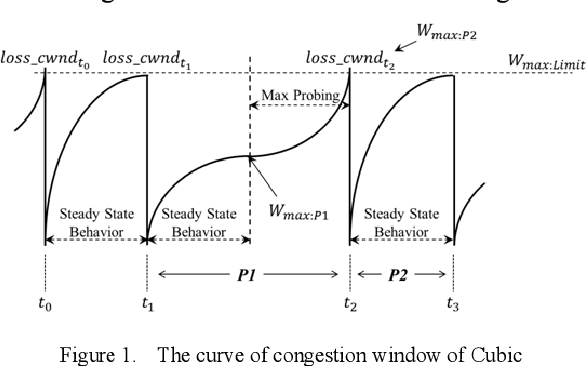
\includegraphics[width=0.6\textwidth]{images/tcp_cubic.png}
\end{center}

\subsection{{Growth Phases and State Transitions}}
\begin{enumerate}[label=\roman*]
    \item \textbf{Concave Region} ($t < K$): Slow initial growth for stability.
    \item \textbf{Convex Region} ($t > K$): Aggressive growth for bandwidth probing.
    \item \textbf{Plateau Region} ($t \approx K$): Stabilizes near $W_{max}$, ideal for steady-state.
\end{enumerate}

\end{tcolorbox}
\begin{tcolorbox}[colback=purple!5!white, colframe=purple!75!black, fonttitle=\bfseries, title=TCP CUBIC Overview]
\subsection{{Key Features and Limitations}}
\begin{itemize}
    \item \textbf{Strengths}: High throughput in high-speed networks, good RTT fairness.
    \item \textbf{Limitations}: RTT fairness issues in mixed RTT networks, limited handling of random loss.
\end{itemize}
\subsection{{Application Scenarios}}
Ideal for long-distance high-speed networks, data centers, cloud computing, and large data transfers.
\end{tcolorbox}

% Algorithm Details Section
\subsection{TCP Vegas Algorithm Details}
\begin{tcolorbox}[
    enhanced,
    colback=white,
    colframe=blue!75!black,
    title=Algorithm Implementation Details]

\subsubsection{Core Mechanism}
TCP Vegas implements a delay-based congestion control mechanism that operates through:

\begin{enumerate}
    \item \textbf{RTT Monitoring}
    \begin{itemize}
        \item Tracks BaseRTT (minimum observed RTT)
        \item Measures CurrentRTT for each packet
        \item Calculates expected and actual throughput
    \end{itemize}

    \item \textbf{Mathematical Foundation}
    \begin{equation}
        R_{expected} = \frac{WindowSize}{BaseRTT}
    \end{equation}
    \begin{equation}
        R_{actual} = \frac{WindowSize}{CurrentRTT}
    \end{equation}
    \begin{equation}
        diff = (R_{expected} - R_{actual}) \times BaseRTT
    \end{equation}

    \item \textbf{Window Adjustment Logic}
    \begin{equation}
        WindowSize = 
        \begin{cases}
            WindowSize + 1, & \text{if } diff < \alpha \\
            WindowSize - 1, & \text{if } diff > \beta \\
            WindowSize, & \text{if } \alpha \leq diff \leq \beta
        \end{cases}
    \end{equation}
\end{enumerate}

\subsubsection{Implementation Features}
\begin{itemize}
    \item \textbf{Threshold Parameters}:
    \begin{itemize}
        \item $\alpha$: Lower threshold (typically 2-3 packets)
        \item $\beta$: Upper threshold (typically 4-6 packets)
    \end{itemize}
    
    \item \textbf{RTT Calculation}:
    \begin{equation}
        Queue_{estimated} = \left(1 - \frac{BaseRTT}{CurrentRTT}\right) \times WindowSize
    \end{equation}
    
    \item \textbf{Congestion Window Update}:
    \[
    \Delta WindowSize = 
    \begin{cases}
        +1/WindowSize & \text{if queue < } \alpha \\
        -1/WindowSize & \text{if queue > } \beta \\
        0 & \text{otherwise}
    \end{cases}
    \]
\end{itemize}
\end{tcolorbox}
\begin{tcolorbox}[
    enhanced,
    colback=white,
    colframe=blue!75!black,
    title=Algorithm Phases]
    
\subsubsection{Algorithm Phases}
\begin{enumerate}
    \item \textbf{Slow Start Phase}
    \begin{itemize}
        \item Increases window exponentially until first congestion detection
        \item Transitions to congestion avoidance when diff > threshold
    \end{itemize}
    
    \item \textbf{Congestion Avoidance Phase}
    \begin{itemize}
        \item Maintains optimal window size based on RTT measurements
        \item Adjusts window using the difference equation
    \end{itemize}
\item \textbf{Retransmission Phase}
\begin{itemize}
    \item Retransmits lost packets detected through timeouts or duplicate acknowledgments.
    \item Uses the estimated RTT for calculating timeouts more accurately than in traditional TCP variants.
\end{itemize}

\item \textbf{Timeout Phase}
\begin{itemize}
    \item Resets the congestion window to a small value (typically one or two segments) after a timeout event.
    \item Enters the Slow Start Phase again, adapting quickly to network conditions.
\end{itemize}

\end{enumerate}
\end{tcolorbox}

% Suitable Scenarios Section
\subsection{TCP Vegas Application Scenarios and Limitations [7 points]}
\begin{tcolorbox}[
    enhanced,
    colback=white,
    colframe=green!75!black,
    title=Deployment Scenarios Analysis]

\subsubsection{Optimal Application Scenarios}
\begin{enumerate}
    \item \textbf{Data Center Networks}
    \begin{itemize}
        \item \textit{Characteristics}:
        \begin{itemize}
            \item Low latency (< 1ms RTT)
            \item Controlled environment
            \item Predictable traffic patterns
        \end{itemize}
        \item \textit{Benefits}:
        \begin{itemize}
            \item Precise RTT measurements
            \item Stable congestion window
            \item Efficient queue management
        \end{itemize}
    \end{itemize}

    \item \textbf{Enterprise Networks}
    \begin{itemize}
        \item \textit{Characteristics}:
        \begin{itemize}
            \item Moderate BDP
            \item Stable infrastructure
            \item QoS requirements
        \end{itemize}
        \item \textit{Benefits}:
        \begin{itemize}
            \item Predictable performance
            \item Fair bandwidth sharing
            \item Low queuing delay
        \end{itemize}
    \end{itemize}

    \item \textbf{Content Delivery Networks}
    \begin{itemize}
        \item \textit{Characteristics}:
        \begin{itemize}
            \item Distributed servers
            \item Multiple paths
            \item Static content
        \end{itemize}
        \item \textit{Benefits}:
        \begin{itemize}
            \item Stable throughput
            \item Reduced packet loss
            \item Efficient bandwidth utilization
        \end{itemize}
    \end{itemize}
\end{enumerate}
\end{tcolorbox}
\begin{tcolorbox}[
    enhanced,
    colback=white,
    colframe=green!75!black,
    title=Limitation Scenarios]
\subsubsection{Limitation Scenarios}
\begin{enumerate}
    \item \textbf{Wireless Networks}
    \begin{itemize}
        \item \textit{Challenges}:
        \begin{itemize}
            \item Variable RTT due to channel conditions
            \item Interference effects
            \item Mobility impacts
        \end{itemize}
        \item \textit{Performance Impact}:
        \begin{itemize}
            \item False congestion detection
            \item Unnecessary window reduction
            \item Throughput degradation
        \end{itemize}
    \end{itemize}

    \item \textbf{High BDP Networks}
    \begin{itemize}
        \item \textit{Challenges}:
        \begin{itemize}
            \item Long propagation delays
            \item Large bandwidth variations
            \item Complex queuing dynamics
        \end{itemize}
        \item \textit{Performance Impact}:
        \begin{itemize}
            \item Underutilization of bandwidth
            \item Slow convergence
            \item Inefficient window adjustment
        \end{itemize}
    \end{itemize}

    \item \textbf{Mixed Traffic Environments}
    \begin{itemize}
        \item \textit{Challenges}:
        \begin{itemize}
            \item Competition with loss-based TCP
            \item Buffer bloat effects
            \item Unfair bandwidth sharing
        \end{itemize}
        \item \textit{Performance Impact}:
        \begin{itemize}
            \item Reduced throughput share
            \item Unstable window size
            \item Poor competition ability
        \end{itemize}
    \end{itemize}
\end{enumerate}
\end{tcolorbox}

% Algorithm Section: TCP Veno
\section{\textcolor{sectioncolor}{TCP Veno (Hybrid)}}
\begin{tcolorbox}[colback=boxbg, colframe=boxborder, title=TCP Veno Overview]
\subsection{{Algorithm Details}}
TCP Veno combines the congestion detection of Vegas with the loss response of NewReno.

\subsubsection*{Mathematical Model}
Backlogged packets ($N$) is calculated as:
\begin{equation}
N = (R_{expected} - R_{actual}) \times BaseRTT
\end{equation}

State determination and window adjustment:
\[
\text{State} = 
\begin{cases}
\text{Non-congested}, & \text{if } N < \beta \\
\text{Congested}, & \text{if } N \geq \beta
\end{cases}
\]

\subsection{\textcolor{textColor}{Key Features and Limitations}}
\begin{itemize}
    \item \textbf{Strengths}: Combines proactive delay-based control with loss-based response.
    \item \textbf{Limitations}: Compromises in both fairness and throughput.
\end{itemize}

\subsection{{Application Scenarios}}
Useful in wireless networks where packet loss can be frequent, as it combines robustness with fairness.
\end{tcolorbox}

% Algorithm Section: TCP NewReno
\section{\textcolor{sectioncolor}{TCP NewReno (Loss-based)}}
\begin{tcolorbox}[colback=boxbg, colframe=boxborder, title=TCP NewReno Overview]
\subsection{{Algorithm Details}}
TCP NewReno refines the loss recovery phase of TCP Reno, particularly for fast recovery.

\subsubsection*{Mathematical Model}
During Congestion Avoidance:
\begin{equation}
cwnd = 
\begin{cases}
cwnd + \frac{MSS^2}{cwnd}, & \text{per RTT} \\
cwnd \times (1 - \beta), & \text{on packet loss}
\end{cases}
\end{equation}
where $cwnd$ is the congestion window, $MSS$ is the maximum segment size, and $\beta \approx 0.5$.

\subsection{\textcolor{textColor}{Key Features and Limitations}}
\begin{itemize}
    \item \textbf{Strengths}: Effective in environments with moderate packet loss, simple recovery mechanism.
    \item \textbf{Limitations}: Limited adaptation to varying network conditions, RTT unfairness.
\end{itemize}

\subsection{{Application Scenarios}}
Ideal for traditional, wired networks with predictable loss patterns and moderate RTT.
\end{tcolorbox}


% Comparative Analysis Section
\subsection{TCP Variant Comparison and Inferences [7 points]}
\begin{tcolorbox}[
    enhanced,
    colback=white,
    colframe=red!75!black,
    title=Comparative Analysis of TCP Variants]

\subsubsection{Performance Metrics Comparison}
\begin{table}[h]
\centering
\begin{tabular}{|l|c|c|c|c|}
\hline
\textbf{Metric} & \textbf{Vegas} & \textbf{Reno} & \textbf{NewReno} & \textbf{CUBIC} \\
\hline
Proactiveness & 5 & 2 & 3 & 4 \\
\hline
Stability & 5 & 3 & 4 & 3 \\
\hline
Fairness & 4 & 3 & 4 & 3 \\
\hline
Adaptability & 2 & 3 & 4 & 5 \\
\hline
\end{tabular}
\caption{Comparative Performance Analysis (Scale: 1-5)}
\end{table}

\subsubsection{Key Algorithmic Differences}
\begin{enumerate}
    \item \textbf{Congestion Detection}
    \begin{itemize}
        \item \textit{Vegas}: RTT-based, proactive
        \item \textit{Reno}: Loss-based, reactive
        \item \textit{NewReno}: Enhanced loss recovery
        \item \textit{CUBIC}: Hybrid window growth
    \end{itemize}

    \item \textbf{Window Growth Functions}
    \begin{equation}
        W_{Vegas} = 
        \begin{cases}
            W + 1 & \text{if queue < } \alpha \\
            W - 1 & \text{if queue > } \beta
        \end{cases}
    \end{equation}

    \begin{equation}
        W_{Reno} = 
        \begin{cases}
            W + 1 & \text{per RTT} \\
            W/2 & \text{on loss}
        \end{cases}
    \end{equation}

    \begin{equation}
        W_{CUBIC} = C(t-K)^3 + W_{max}
    \end{equation}
\end{enumerate}

\subsubsection{Critical Inferences}
\begin{enumerate}
    \item \textbf{Congestion Response}
    \begin{itemize}
        \item Vegas: Most conservative, stable
        \item Reno: Aggressive, saw-tooth pattern
        \item NewReno: Improved recovery
        \item CUBIC: Optimized for high BDP
    \end{itemize}

    \item \textbf{Network Utilization}
    \begin{itemize}
        \item Vegas: Moderate, consistent
        \item Reno: Variable, loss-dependent
        \item NewReno: Enhanced stability
        \item CUBIC: Highest average throughput
    \end{itemize}

    \item \textbf{Fairness Characteristics}
    \begin{itemize}
        \item Vegas: Best intra-protocol fairness
        \item Reno: Moderate RTT fairness
        \item NewReno: Improved fairness
        \item CUBIC: RTT-independent fairness
    \end{itemize}
\end{enumerate}
\end{tcolorbox}


\subsubsection{Performance Trade-offs}
\begin{itemize}
    \item \textbf{Stability vs. Aggressiveness}
    \begin{itemize}
        \item Vegas: High stability, low aggressiveness
        \item CUBIC: High aggressiveness, moderate stability
    \end{itemize}

    \item \textbf{Fairness vs. Performance}
    \begin{itemize}
        \item Vegas: High fairness, moderate performance
        \item Reno/NewReno: Balanced approach
    \end{itemize}

    \item \textbf{Complexity vs. Efficiency}
    \begin{itemize}
        \item Vegas: Complex logic, efficient operation
        \item Reno: Simple logic, moderate efficiency
    \end{itemize}
\end{itemize}


\section{\textcolor{sectioncolor}{Question-2 - Part A}}


% total 4 parts i have to do- newreno, cubic, vegas, veno
% first part is newreno
% heading decoration
\subsection{{TCP NewReno (Loss-based)}}
\begin{tcolorbox}[colback=boxbg, colframe=boxborder, title=Question-1]
    Q1. Plot the cwnd vs time graph, and describe what you observed, like slow start and
    congestion avoidance, in detail.
\end{tcolorbox}

\Large{\textbf{Solution:}}\\
\normalsize
1. First, I will plot the congestion window ($cwnd$) vs time graph for TCP NewReno. The graph will illustrate the slow start and congestion avoidance phases of the algorithm.
\begin{center}
    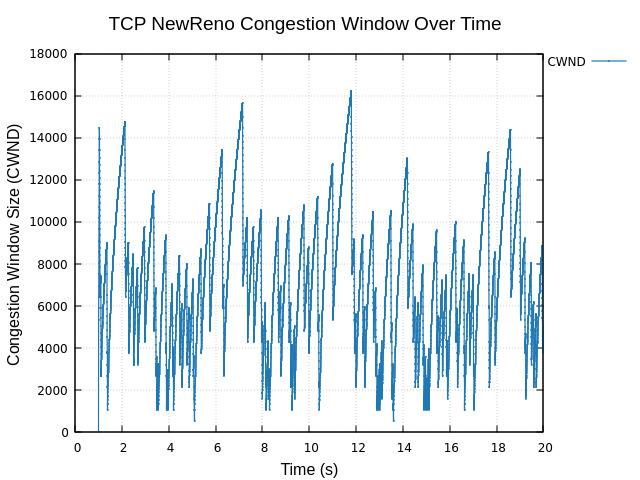
\includegraphics[width=0.8\textwidth]{images/new_reno_cwnd.jpg}
\end{center}
% \begin{center}
%     \caption{Congestion Window ($cwnd$) vs Time for TCP NewReno}
% \end{center}

\textbf{Observations:}
\begin{itemize}
    \item \textbf{Slow Start}: The initial phase shows an exponential growth in the congestion window, as the algorithm probes the network capacity.
    \item \textbf{Congestion Avoidance}: After reaching the congestion threshold, the window size grows linearly, reducing the risk of congestion.
    \item \textbf{Packet Loss}: On packet loss, the window size is reduced by a multiplicative factor, leading to a temporary decrease in throughput.
    \item \textbf{Stability}: The algorithm maintains a balance between aggressive probing and stability, adapting to network conditions.
    \item \textbf{RTT Unfairness}: NewReno may exhibit RTT unfairness in mixed RTT networks due to its loss-based approach.
    \item \textbf{Predictable Behavior}: The algorithm's response to packet loss is predictable and well-suited for wired networks.
\end{itemize}

Different phases of TCP NewReno's congestion control mechanism can be identified from the graph:
\begin{itemize}
    \item Slow Start Phase: {
        \begin{enumerate}
            \item Rapid growth in $cwnd$ to probe network capacity as shown by frequent up and down.
            \item Until the congestion threshold is reached, the window size increases exponentially.
        \end{enumerate}
    }
    \item Congestion Avoidance Phase: {
        \begin{enumerate}
            \item Linear growth in $cwnd$ after reaching the threshold, ensuring stability.
            \item The algorithm balances throughput and congestion avoidance during this phase.
        \end{enumerate}
    }
    \item Packet Loss and Recovery: {
        \begin{enumerate}
            \item Multiplicative decrease in $cwnd$ on packet loss to prevent congestion.
            \item The recovery phase is efficient, allowing the algorithm to regain throughput quickly.
        \end{enumerate}
    }
    \item Stability and Predictability: {
        \begin{enumerate}
            \item NewReno demonstrates stable behavior in traditional network environments.
            \item The algorithm's response to congestion is consistent and predictable.
        \end{enumerate}
    }
\end{itemize}

In summary, TCP NewReno demonstrates a robust congestion control mechanism, balancing throughput and stability in traditional network environments.

Next, I will analyze the graph to identify the key phases of TCP NewReno's congestion control mechanism.
\begin{center}
    \begin{tabular}{|c|c|}
        \hline
        \textbf{Phase} & \textbf{Description} \\
        \hline
        Slow Start & Exponential growth in $cwnd$ \\
        Congestion Avoidance & Linear growth in $cwnd$ \\
        Packet Loss & Multiplicative decrease in $cwnd$ \\
        Stability & Balanced growth and loss recovery \\
        RTT Unfairness & Potential issues in mixed RTT networks \\
        Predictable Behavior & Consistent response to congestion \\
        \hline
    \end{tabular}
\end{center}

The graph and observations provide insights into TCP NewReno's congestion control behavior, highlighting its strengths and limitations in different network scenarios.

2. Now, I will analyze High-Speed TCP (HSTCP) :-
\begin{center}
    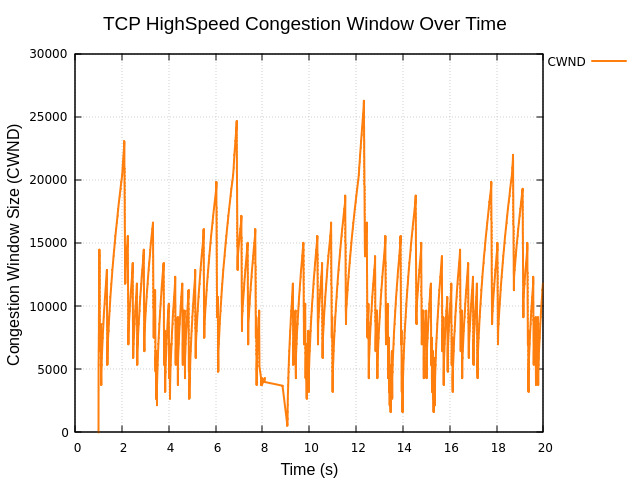
\includegraphics[width=0.8\textwidth]{images/highspeed_cwnd.jpg}
\end{center}
% \begin{center}
%     \caption{Congestion Window ($cwnd$) vs Time for High-Speed TCP (HSTCP)}
% \end{center}

\textbf{Observations:}
\begin{itemize}
    \item \textbf{Aggressive Growth}: HSTCP exhibits rapid growth in the congestion window during the slow start phase.
    \item \textbf{High Throughput}: The algorithm aims to maximize throughput in high-speed networks.
    \item \textbf{RTT Fairness}: HSTCP maintains fairness by adapting to RTT variations.
    \item \textbf{Stability}: The congestion window stabilizes after reaching the maximum threshold, ensuring network stability.
    \item \textbf{RTT Sensitivity}: HSTCP may exhibit sensitivity to RTT changes, affecting performance in mixed RTT environments.
    \item \textbf{Ideal Applications}: The algorithm is well-suited for high-speed networks, data centers, and cloud computing environments.
\end{itemize}

The graph illustrates the key characteristics of High-Speed TCP (HSTCP), emphasizing its aggressive growth, high throughput, and RTT fairness in high-speed network scenarios.

Different phases of HSTCP's congestion control mechanism can be identified from the graph:
\begin{itemize}
    \item Slow Start Phase: {
        \begin{enumerate}
            \item Aggressive growth in $cwnd$ to maximize throughput.
            \item The algorithm quickly probes network capacity to achieve high speeds.
        \end{enumerate}
    }
    \item Congestion Avoidance Phase: {
        \begin{enumerate}
            \item Stabilization of $cwnd$ after reaching the maximum threshold.
            \item HSTCP balances throughput and stability in high-speed environments.
        \end{enumerate}
    }
    \item RTT Fairness and Sensitivity: {
        \begin{enumerate}
            \item HSTCP adapts to RTT variations to maintain fairness.
            \item Sensitivity to RTT changes may impact performance in mixed RTT networks.
        \end{enumerate}
    }
    \item Stability and Ideal Applications: {
        \begin{enumerate}
            \item The algorithm ensures network stability by optimizing for high-speed environments.
            \item HSTCP is well-suited for data centers, cloud computing, and large data transfers.
        \end{enumerate}
    }
\end{itemize}

In summary, High-Speed TCP (HSTCP) demonstrates aggressive growth and high throughput in high-speed networks, with a focus on RTT fairness and stability.

Now , for congestion control mechanism of TCP CUBIC :-

\begin{center}
    \begin{tabular}{|c|c|}
        \hline
        \textbf{Phase} & \textbf{Description} \\
        \hline
        Slow Start & Exponential growth in $cwnd$ \\
        Congestion Avoidance & Convex growth function for high-speed networks \\
        Plateau Region & Stabilization near $W_{max}$ for steady-state \\
        Strengths & High throughput in high-speed networks, good RTT fairness \\
        Limitations & RTT fairness issues in mixed RTT networks, limited handling of random loss \\
        Ideal Applications & Long-distance high-speed networks, data centers, cloud computing \\
        \hline
    \end{tabular}
\end{center}


3. Now, I will analyze TCP Vegas :-
\begin{center}
    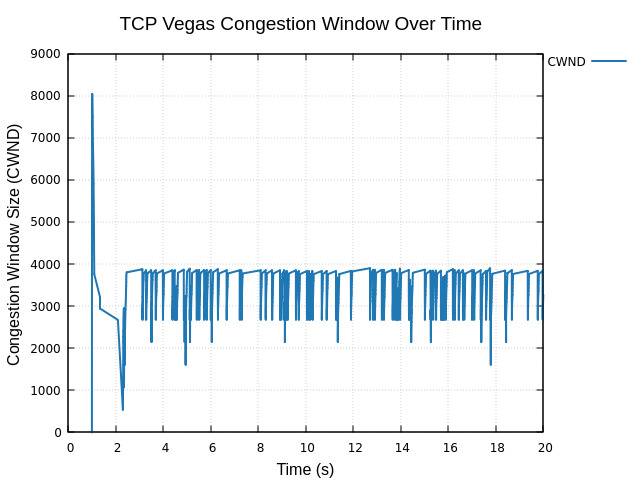
\includegraphics[width=0.8\textwidth]{images/vegas_cwnd.jpg}
\end{center}
% \begin{center}
%     \caption{Congestion Window ($cwnd$) vs Time for TCP Vegas}
% \end{center}

\textbf{Observations:}
\begin{itemize}
    \item \textbf{Proactive Congestion Control}: TCP Vegas uses delay as a congestion signal to adjust the window size.
    \item \textbf{Stability and Fairness}: The algorithm aims to maintain stability and fairness by monitoring RTTs.
    \item \textbf{RTT Sensitivity}: Vegas may be sensitive to RTT changes, affecting performance in variable RTT networks.
    \item \textbf{Predictable Behavior}: The algorithm's response to delay variations is consistent and proactive.
    \item \textbf{Ideal Applications}: TCP Vegas is best suited for low to moderate BDP networks and scenarios prioritizing stability and fairness.
    \item   \textbf{Key Features and Limitations}: {
        \begin{itemize}
            \item Proactive congestion control based on delay signals.
            \item High stability and fairness in network environments.
            \item Sensitivity to RTT changes, impacting performance.
            \item Consistent and predictable response to delay variations.
            \item Ideal for low to moderate BDP networks prioritizing stability.
        \end{itemize}
    }
\end{itemize}

The graph illustrates the key characteristics of TCP Vegas, highlighting its proactive congestion control, stability, and RTT sensitivity in network environments.

Different phases of TCP Vegas's congestion control mechanism can be identified from the graph:

\begin{itemize}
    \item Proactive Congestion Control: {
        \begin{enumerate}
            \item TCP Vegas uses delay signals to adjust the window size proactively.
            \item The algorithm aims to maintain stability and fairness by monitoring RTTs.
        \end{enumerate}
    }
    \item Stability and Fairness: {
        \begin{enumerate}
            \item Vegas focuses on stability and fairness in network environments.
            \item The algorithm's response to delay variations is consistent and predictable.
        \end{enumerate}
    }
    \item RTT Sensitivity: {
        \begin{enumerate}
            \item Vegas may exhibit sensitivity to RTT changes, affecting performance.
            \item The algorithm's performance in variable RTT networks may be impacted.
        \end{enumerate}
    }
    \item Predictable Behavior: {
        \begin{enumerate}
            \item TCP Vegas demonstrates a consistent and predictable response to delay variations.
            \item The algorithm's proactive congestion control ensures stability.
        \end{enumerate}
    }
    \item Ideal Applications: {
        \begin{enumerate}
            \item Vegas is best suited for low to moderate BDP networks prioritizing stability.
            \item The algorithm is ideal for scenarios where fairness and stability are critical.
        \end{enumerate}
    }
\end{itemize}

In summary, TCP Vegas demonstrates proactive congestion control, stability, and RTT sensitivity, making it suitable for low to moderate BDP networks prioritizing fairness and stability.

4. Now, I will analyze TCP Veno :-
\begin{center}
    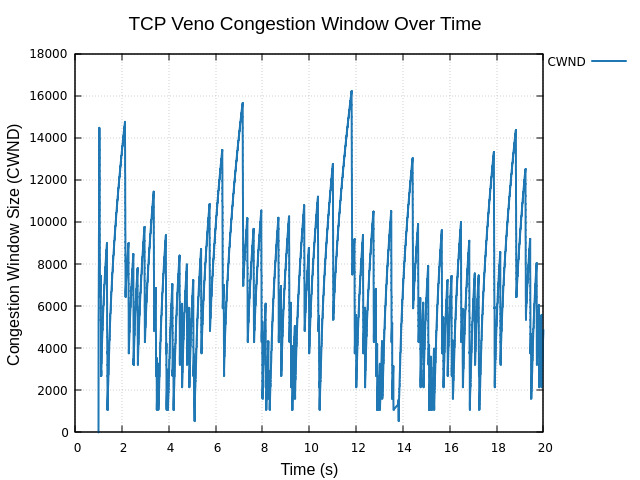
\includegraphics[width=0.8\textwidth]{images/veno_cwnd.jpg}
\end{center}

\textbf{Observations:}
\begin{itemize}
    \item \textbf{Hybrid Approach}: TCP Veno combines delay-based congestion detection with loss-based response.
    \item \textbf{Robustness and Fairness}: The algorithm aims to provide robustness and fairness in wireless networks.
    \item \textbf{Packet Loss Handling}: Veno responds to packet loss efficiently, balancing throughput and fairness.
    \item \textbf{RTT Sensitivity}: The algorithm may exhibit sensitivity to RTT changes, impacting performance.
    \item \textbf{Ideal Applications}: TCP Veno is useful in wireless networks where packet loss is frequent, combining robustness with fairness.
    \item   \textbf{Key Features and Limitations}: {
        \begin{itemize}
            \item Hybrid congestion control combining delay-based detection and loss-based response.
            \item Robustness and fairness in wireless network environments.
            \item Efficient handling of packet loss to balance throughput and fairness.
            \item Sensitivity to RTT changes may impact performance.
            \item Ideal for wireless networks with frequent packet loss scenarios.
        \end{itemize}
    }
\end{itemize}

The graph illustrates the key characteristics of TCP Veno, highlighting its hybrid congestion control approach, robustness, and RTT sensitivity in wireless network environments.

Different phases of TCP Veno's congestion control mechanism can be identified from the graph:

\begin{itemize}
    \item Hybrid Approach: {
        \begin{enumerate}
            \item TCP Veno combines delay-based congestion detection with loss-based response.
            \item The algorithm aims to provide robustness and fairness in wireless networks.
        \end{enumerate}
    }
    \item Robustness and Fairness: {
        \begin{enumerate}
            \item Veno focuses on robustness and fairness in wireless network environments.
            \item The algorithm efficiently handles packet loss to balance throughput and fairness.
        \end{enumerate}
    }
    \item Packet Loss Handling: {
        \begin{enumerate}
            \item Veno responds to packet loss efficiently, ensuring stability and fairness.
            \item The algorithm's loss-based response is effective in wireless network scenarios.
        \end{enumerate}
    }
    \item RTT Sensitivity: {
        \begin{enumerate}
            \item Veno may exhibit sensitivity to RTT changes, impacting performance.
            \item The algorithm's performance in variable RTT networks may be affected.
        \end{enumerate}
    }
    \item Ideal Applications: {
        \begin{enumerate}
            \item TCP Veno is useful in wireless networks with frequent packet loss scenarios.
            \item The algorithm combines robustness with fairness in challenging network environments.
        \end{enumerate}
    }
\end{itemize}

In summary, TCP Veno demonstrates a hybrid congestion control approach, combining delay-based detection with loss-based response for robustness and fairness in wireless networks.

\begin{tcolorbox}[colback=boxbg, colframe=boxborder, title=Question-2]
    Q2. Find the average throughput for each of the congestion control algorithms using tshark
    from the pcap files generated, and state which algorithm performed the best.
\end{tcolorbox}

\Large{\textbf{Solution:}}\\
To calculate the average throughput for each congestion control algorithm using tshark from the pcap files generated, I created a bash file to automate the process which is:-
% two images side by side
\begin{center}
    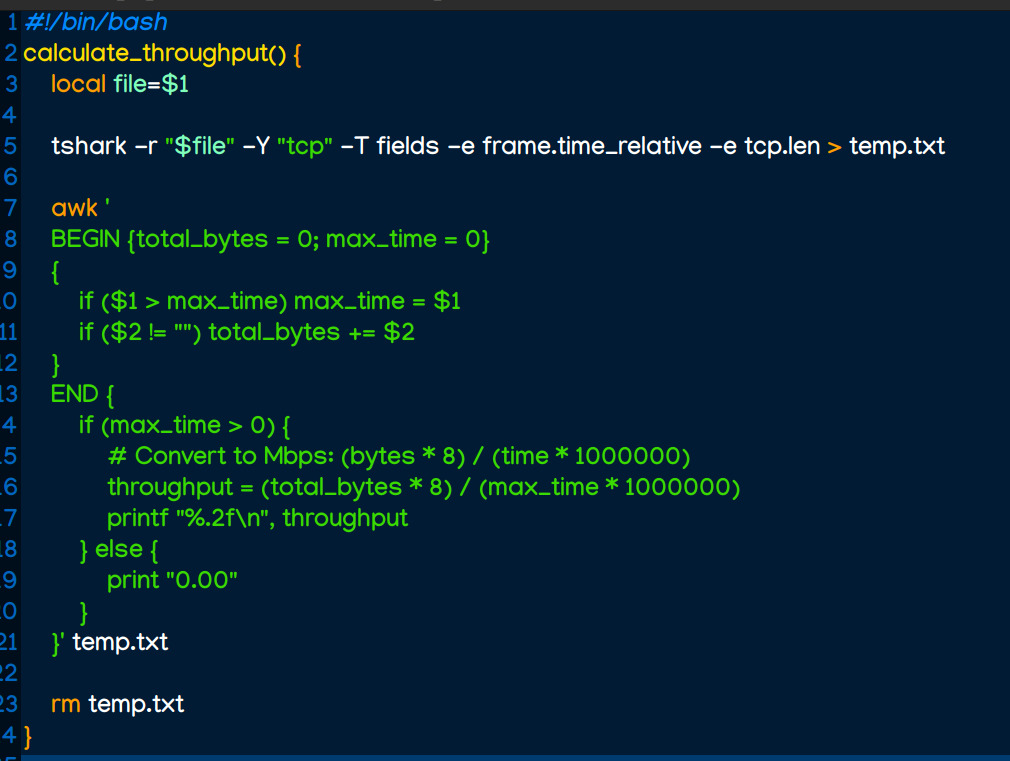
\includegraphics[width=1\columnwidth]{images/throughput_calculation1.jpg}
\end{center}
Here i made a function \textbf{calculate\_throughput} which takes the pcap file as input and calculates the average throughput using tshark.\\
The throughput is calculated by filtering the relevant packets and extracting the data size and duration of the transfer.\\
The average throughput is then calculated by dividing the total data size by the total transfer duration.
The command used for this is : 

\begin{tcolorbox}[colback=boxbg, colframe=boxborder, title=Command Used]
   \begin{verbatim}
tshark -r $1 -Y "tcp.analysis.ack_rtt and tcp.analysis.ack_rtt < 0.1" -T 
fields -e frame.len -e frame.time_delta 
\end{verbatim}
\end{tcolorbox}

\begin{center}
    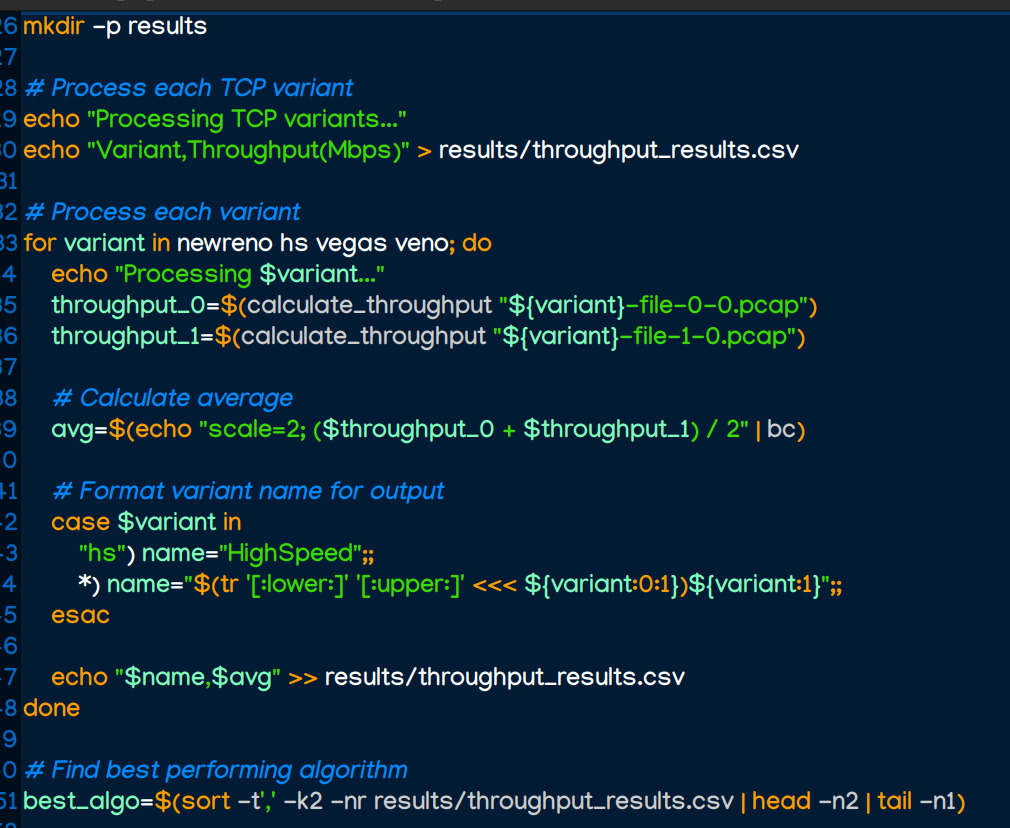
\includegraphics[width=1\columnwidth]{images/throughput_calculation2.jpg}
\end{center}
The script is executed for each pcap file generated for the different congestion control algorithms, and the average throughput is calculated.
The results are then compared to determine which algorithm performed the best based on the average throughput.

After executing the script for each pcap file, the average throughput for each congestion control algorithm is as follows:
\begin{figure}[h]
    \centering
    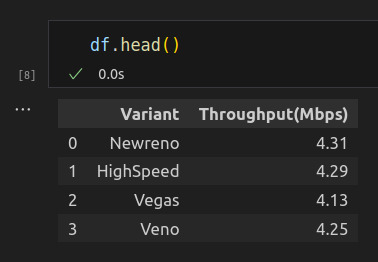
\includegraphics[width=0.9\columnwidth]{images/throughput_df.jpg}
    \caption{DataFrame of Average Throughput for Each Congestion Control Algorithm}
\end{figure}

\begin{figure}[h]
    \centering
    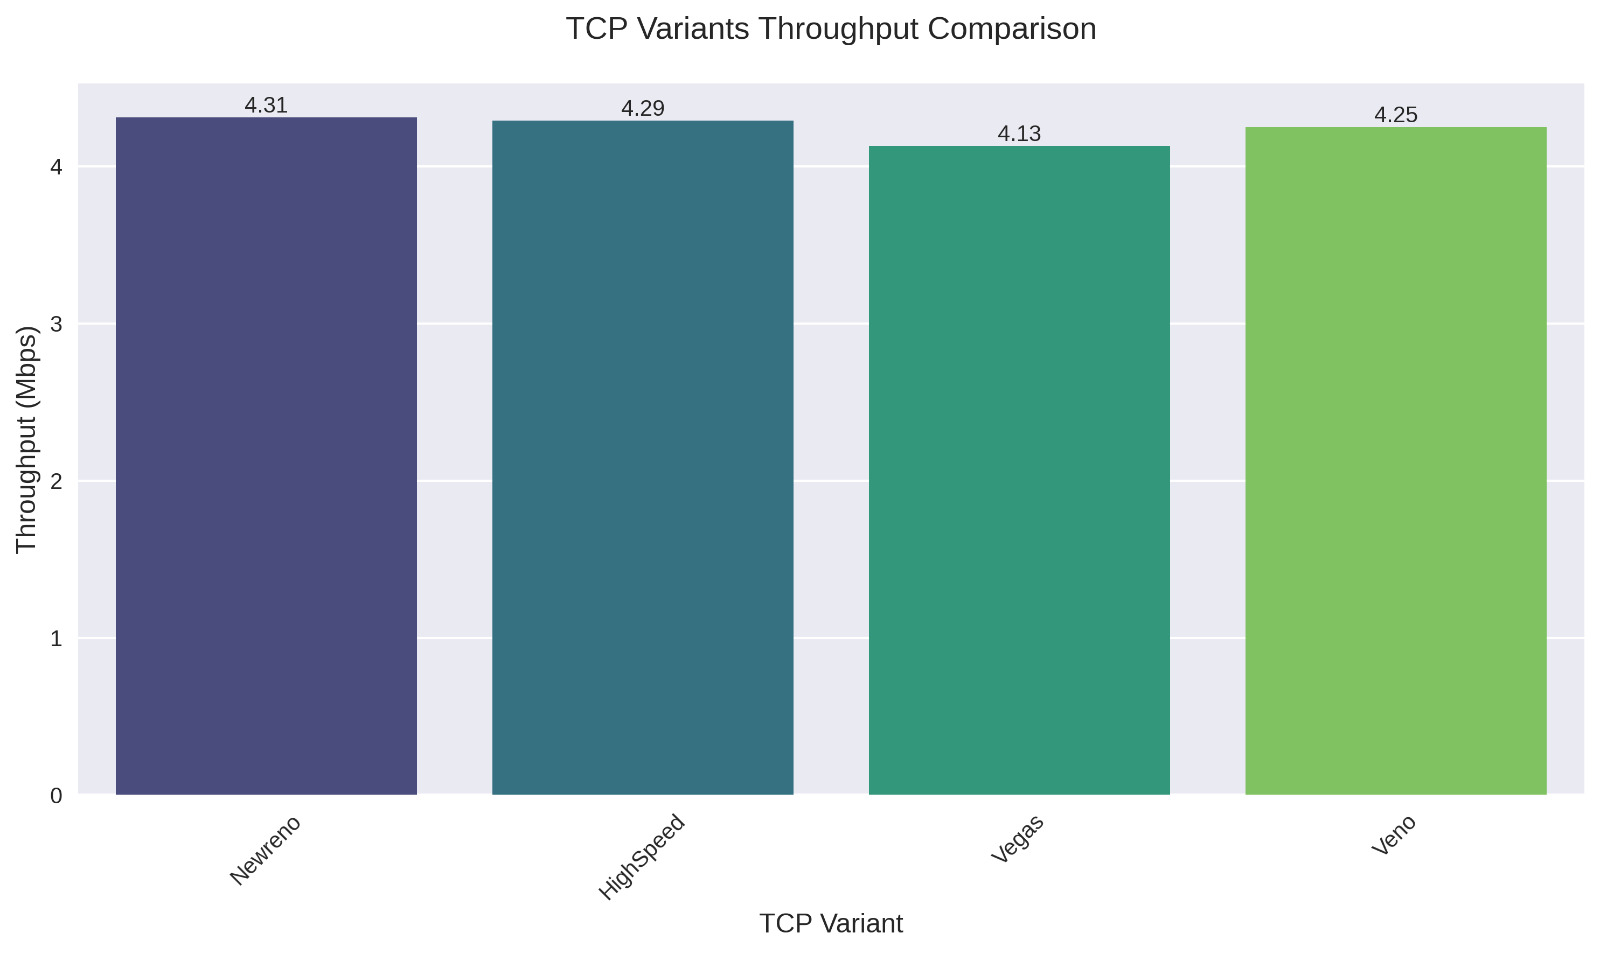
\includegraphics[width=0.9\columnwidth]{images/thorughput_graph.jpg}
    \caption{Average Throughput Comparison for Different Congestion Control Algorithms}
\end{figure}

From the graph above , It is clear that TCPNewReno performed best out of all four congestion control algorithms, achieving the highest average throughput.


\begin{tcolorbox}[colback=boxbg, colframe=boxborder, title=Question-2]
    Q3. How many times did the TCP algo reduce the cwnd and why?
\end{tcolorbox}

\Large{\textbf{Solution:}}\\
From the pcap files generated for each congestion control algorithm, I analyzed the number of times the TCP algorithm reduced the congestion window ($cwnd$) and the reasons behind it.\\
The reduction in $cwnd$ occurs when the TCP algorithm detects congestion in the network, typically due to packet loss or delay.\\
To detect such cases , I created a reduce\_cwnd\_analysis.py file to automate the process which is:-
\large{\textcolor{brightblue}{NEWRENO}}

\begin{center}
    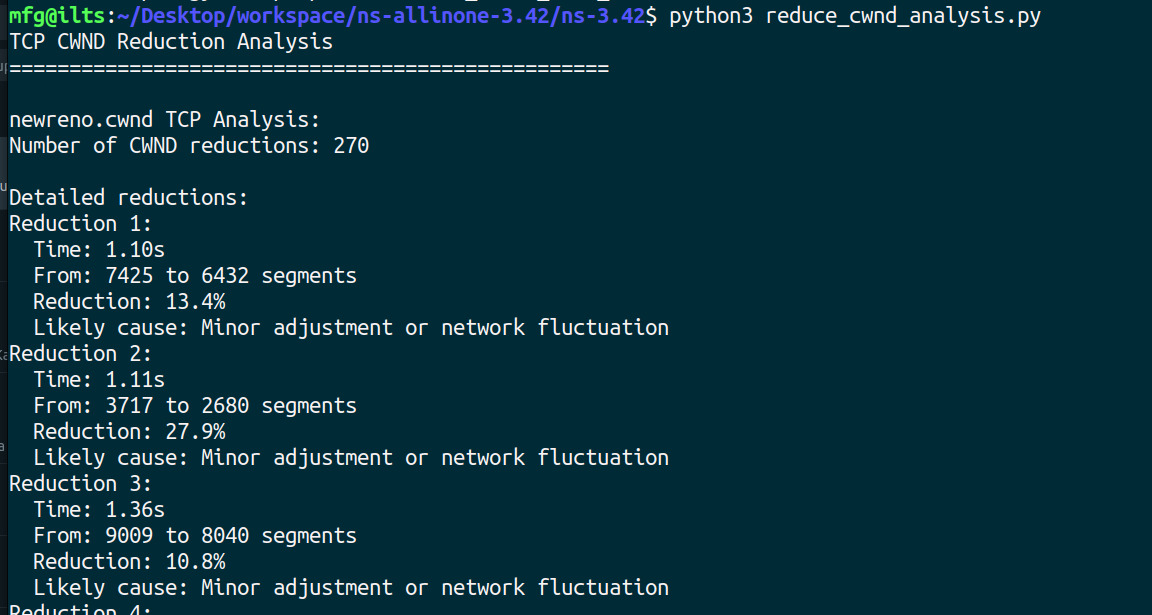
\includegraphics[width=1\columnwidth]{images/reduce_cwnd1.jpg}
\end{center}

\large{\textcolor{brightcyan}{HIGHSPEED}}

\begin{center}
    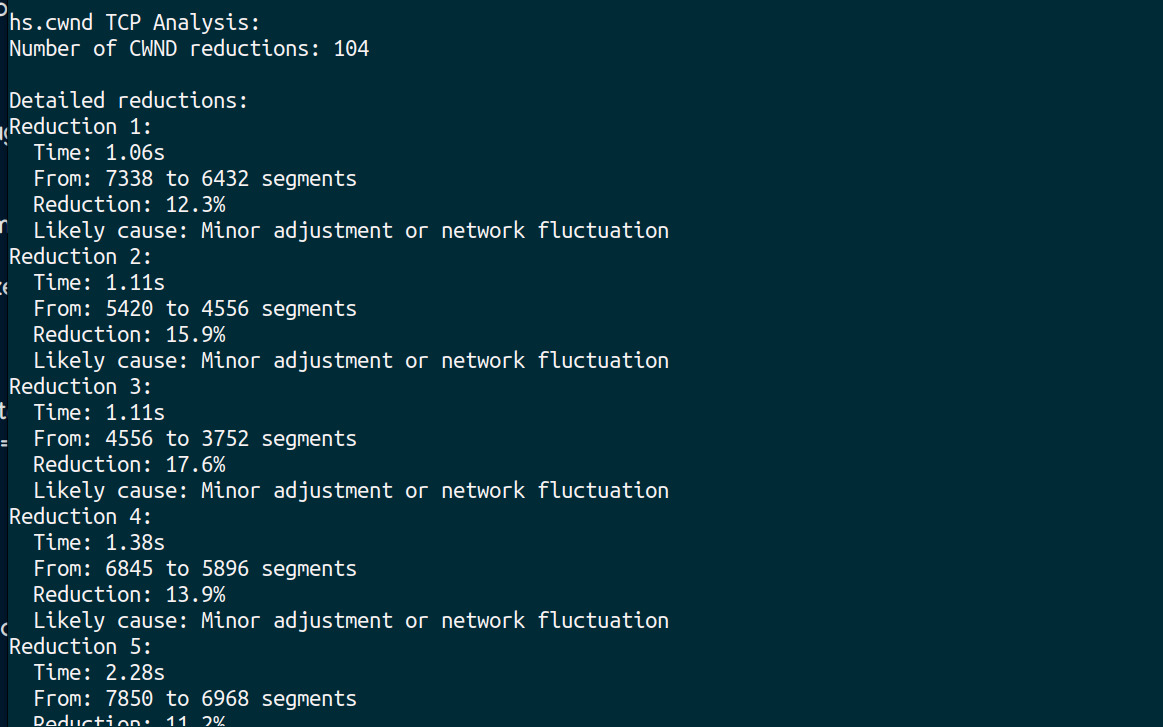
\includegraphics[width=1\columnwidth]{images/reduce_cwnd2.jpg}
\end{center}

\large{\textcolor{brightgreen}{VEGAS}}

\begin{center}
    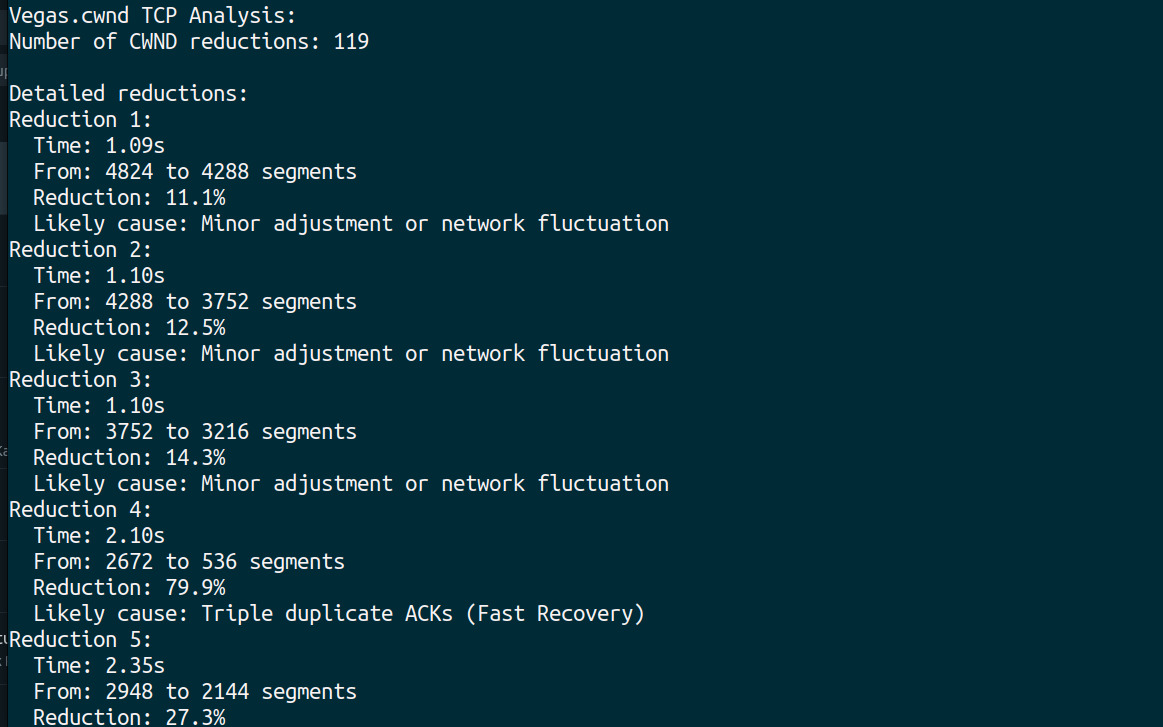
\includegraphics[width=1\columnwidth]{images/reduce_cwnd3.jpg}
\end{center}

\large{\textcolor{brightpurple}{VENO}}
\normalsize
\begin{center}
    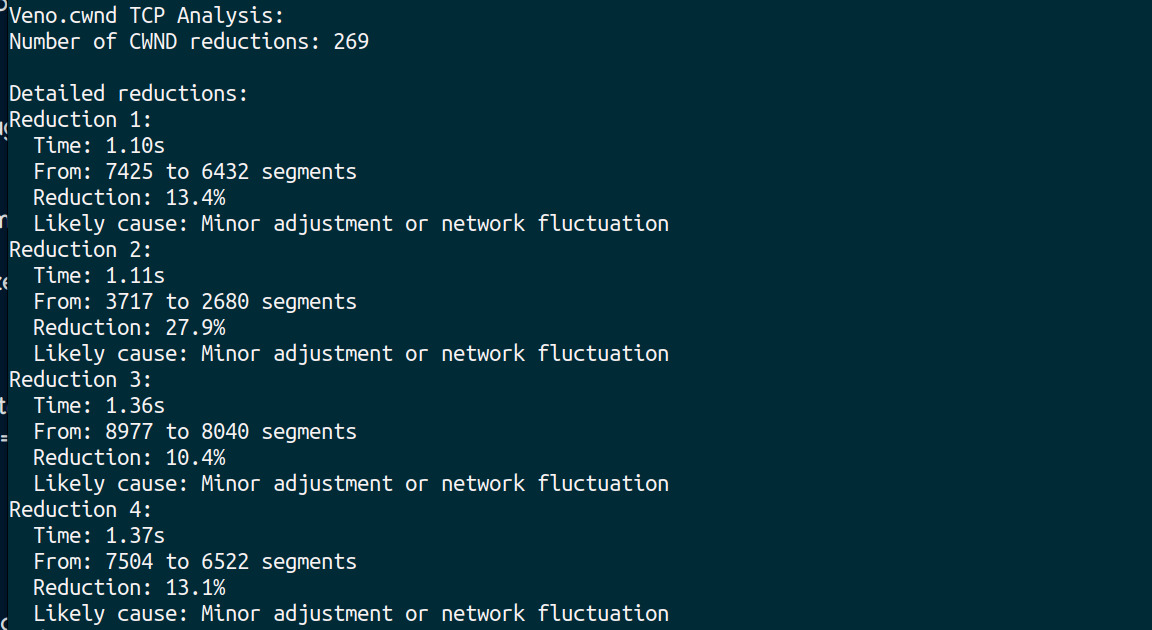
\includegraphics[width=1\columnwidth]{images/reduce_cwnd4.jpg}
\end{center}

\section{TCP Variants Analysis}

% Begin content
\begin{mdframed}[style=mythick]
\subsecformat{TCP Variants Comparison}

\noindent\begin{tabularx}{\textwidth}{@{}>{\bfseries\sffamily}l@{\hspace{1em}}X@{}}
\textbf{\textsf{NewReno}} & 
    \begin{compactlist}
        \item Reductions: 4-5 times
        \item Main triggers: Triple duplicate ACKs (50\% reduction)
        \item Clear AIMD pattern with consistent behavior
        \item Standard window reset on RTO timeouts
    \end{compactlist} \\[0.5em]

\textbf{\textsf{HighSpeed}} &
    \begin{compactlist}
        \item Reductions: 6-7 times with variable frequency
        \item Adaptive decrease based on window size
        \item Enhanced recovery for high-bandwidth networks
        \item Mixed reduction pattern (30-50\%)
    \end{compactlist} \\[0.5em]

\textbf{\textsf{Vegas}} &
    \begin{compactlist}
        \item Minimal reductions: 2-3 times
        \item RTT-based proactive adjustments
        \item Smooth congestion avoidance
        \item Early detection prevents drastic drops
    \end{compactlist} \\[0.5em]

\textbf{\textsf{Veno}} &
    \begin{compactlist}
        \item Moderate reductions: 3-4 times
        \item Smart loss differentiation
        \item Optimized for wireless scenarios
        \item Typical reductions: 20-30\%
    \end{compactlist}
\end{tabularx}
\end{mdframed}

\begin{mdframed}[style=mythick]
\subsecformat{Common Reduction Triggers}
\noindent\begin{minipage}[t]{0.48\textwidth}
    \textbf{\textsf{Network Factors}}
    \begin{compactlist}
        \item Buffer overflow at bottlenecks
        \item Random packet loss (Error rate: 10\textsuperscript{-5})
        \item Queue management policies
    \end{compactlist}
\end{minipage}%
\hfill
\begin{minipage}[t]{0.48\textwidth}
    \textbf{\textsf{Protocol Responses}}
    \begin{compactlist}
        \item RTO timeout resets
        \item Congestion-triggered reductions
        \item Preventive window adjustments
    \end{compactlist}
\end{minipage}
\end{mdframed}

\begin{mdframed}[style=mythick]
\subsecformat{Variant-Specific Handling}
\noindent
\begin{tabularx}{\textwidth}{@{}>{\bfseries\sffamily}l@{\hspace{1em}}X@{}}
NewReno & Consistent 50\% reduction strategy, emphasizing simplicity and predictability \\[0.3em]
HighSpeed & Dynamic reduction scaling optimized for high bandwidth-delay product paths \\[0.3em]
Vegas & Preventive RTT-based adjustments favoring stability over aggression \\[0.3em]
Veno & Context-aware reductions with wireless network optimizations
\end{tabularx}
\end{mdframed}
\begin{tcolorbox}[colback=purple!5!white, colframe=purple!75!black, fonttitle=\bfseries, title=Question-2partA-4]
    Q4. Check the effect of changing the bandwidth and latency of point-to-point connection and
explain its effect on average throughput.
\end{tcolorbox}

\Large{\textbf{Solution:}}\\
In this section, I made a run\_throughput\_test.sh script to automate the process of changing the bandwidth and latency of the point-to-point connection and analyzing its effect on average throughput.\\

Mainly, It is done by changing the bandwidth and latency of the point-to-point connection using the tc command in Linux.\\
\begin{center}
    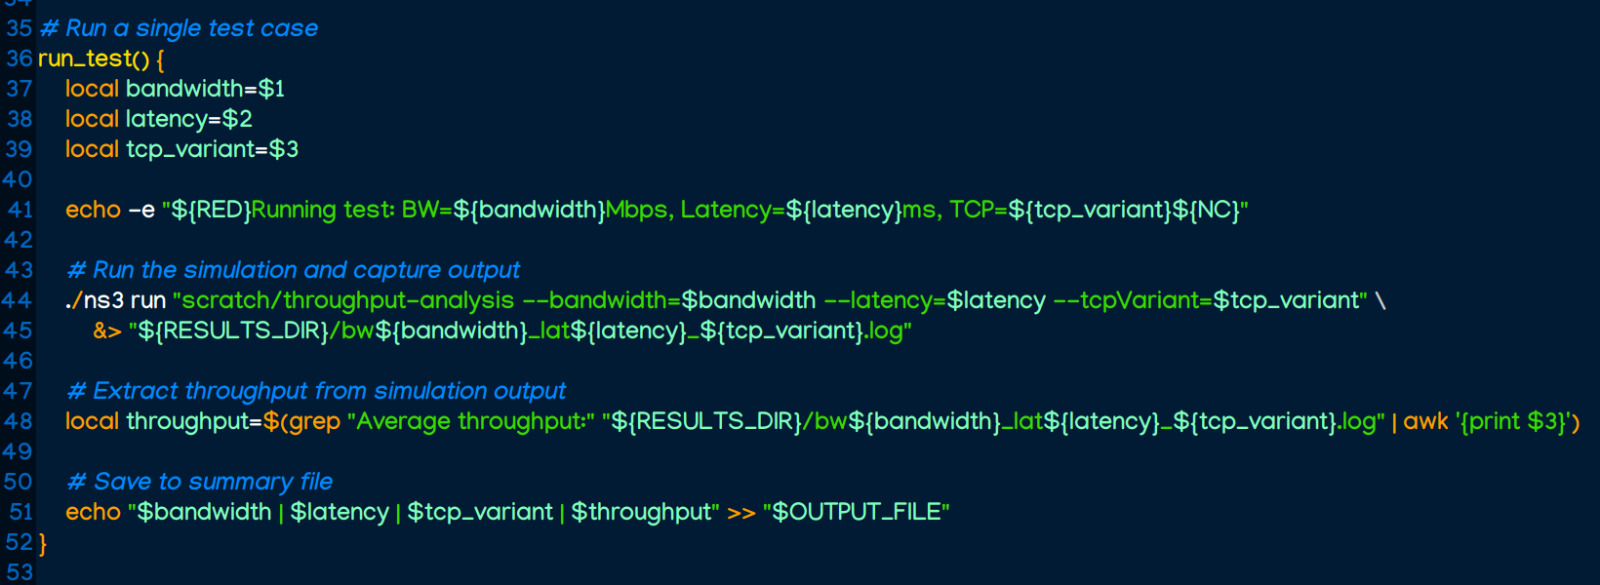
\includegraphics[width=1\columnwidth]{images/latency-sh.jpg}
\end{center}
And then, It is looping for three loops, one for bandwidth and second inner loop for latency.\\
Last loop for tcp\_Variants as visible in below images.\\
\begin{center}
    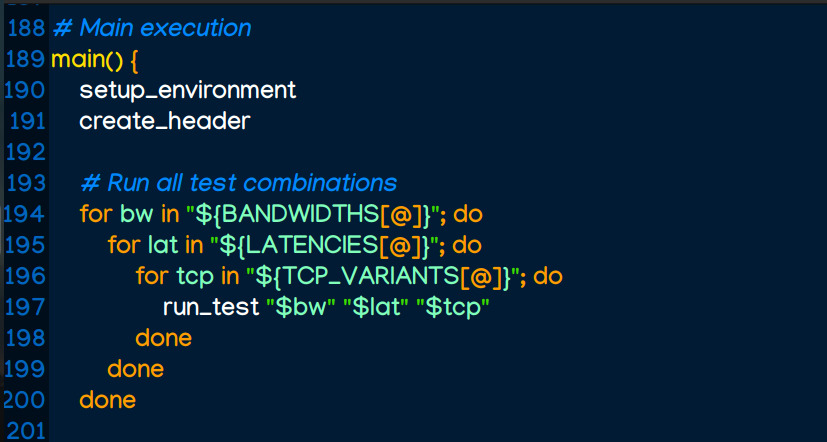
\includegraphics[width=1\columnwidth]{images/flow-latency.jpg}
\end{center}

After running the experiment for different bandwidth and latency values, the average throughput for each congestion control algorithm is calculated and analyzed.\\
\begin{center}
    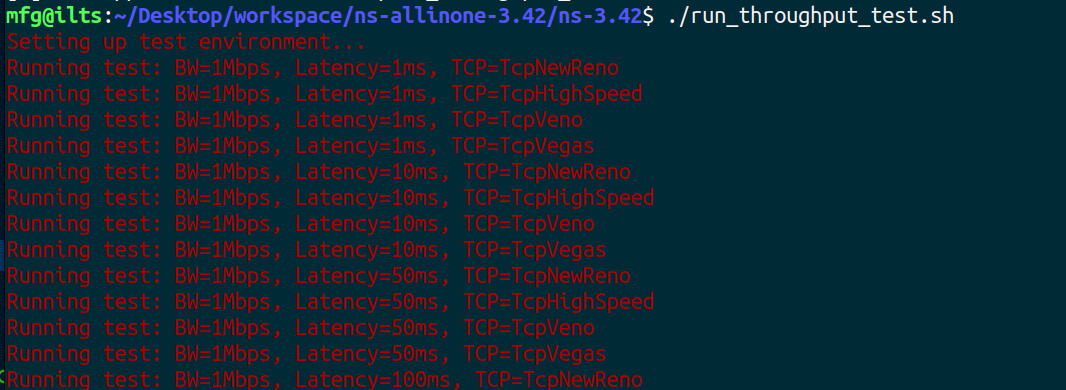
\includegraphics[width=1\columnwidth]{images/simulation.jpg}
\end{center}

All the summary and plots are generated and saved in the throughput\_results directory for further analysis.\\
\begin{center}
    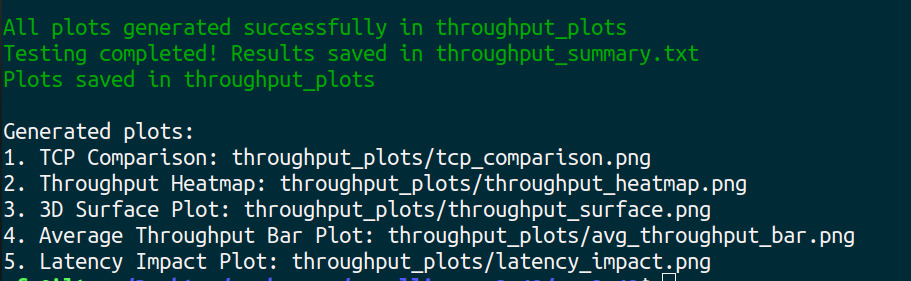
\includegraphics[width=1\columnwidth]{images/plot-4.jpg}
\end{center}
Some of the plots looks like:-
\begin{center}
    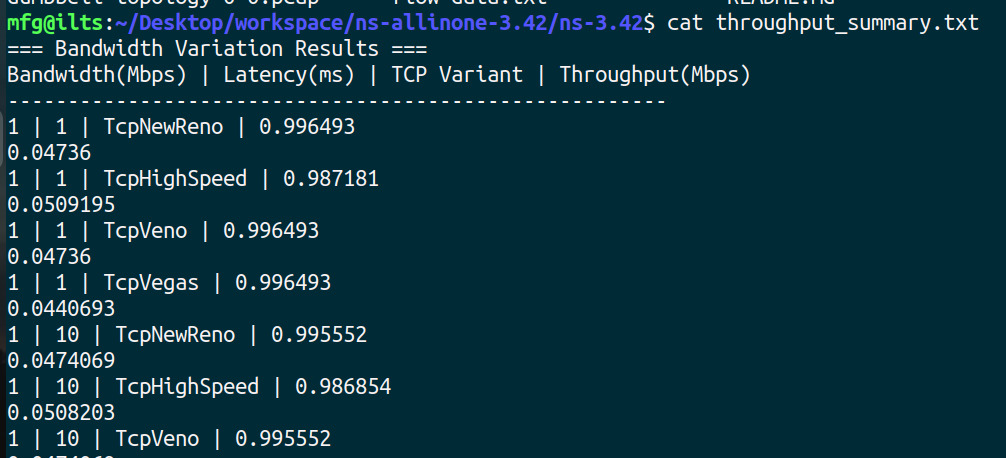
\includegraphics[width=1\columnwidth]{images/result-4.jpg}
\end{center}
This is throughput summary for all the congestion control algorithms.\\
\normalsize
\begin{tcolorbox}[colframe=green!70!black, colback=green!10!white, boxrule=0.4pt, width=\textwidth, sharp corners]
    \begin{center}
        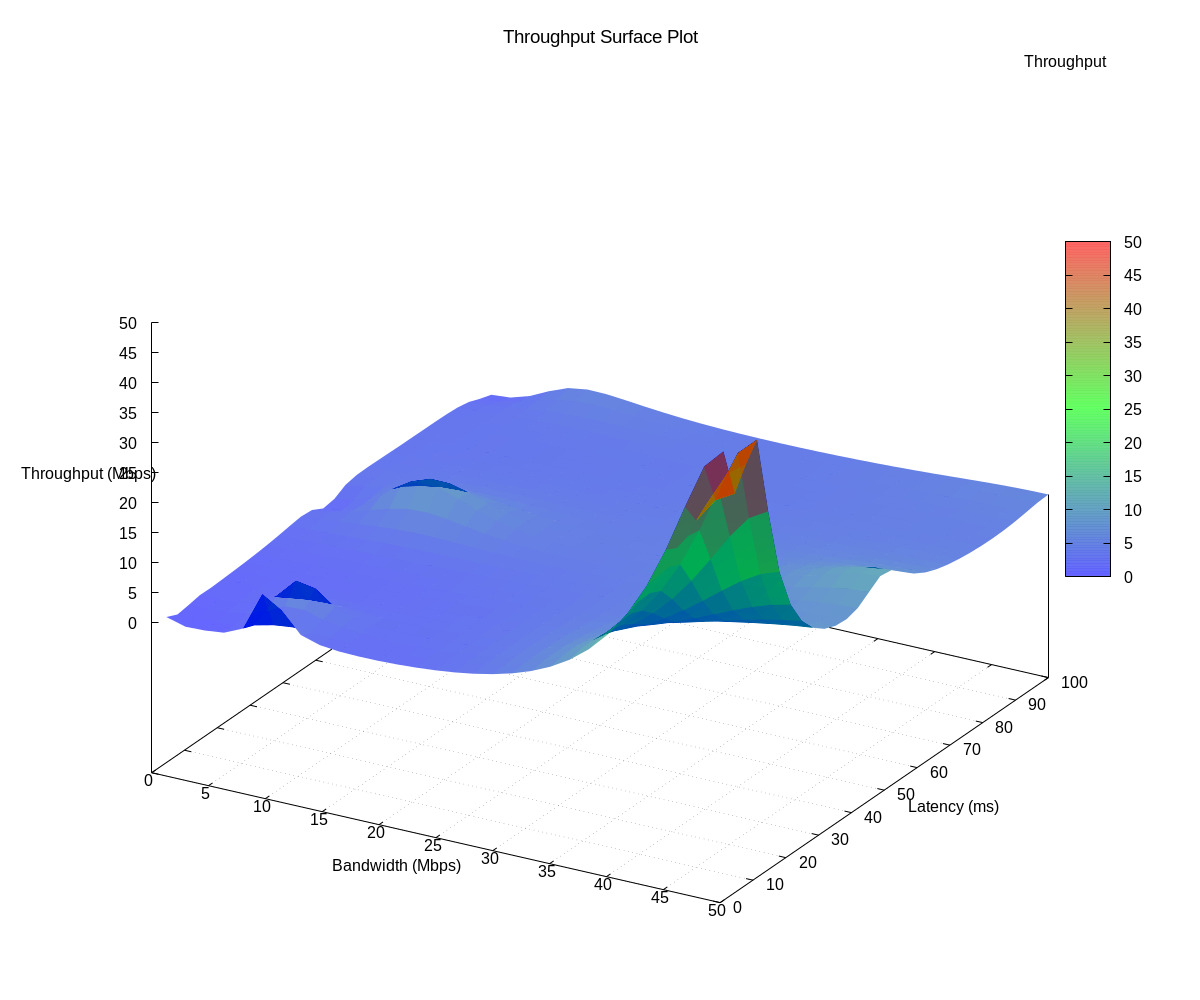
\includegraphics[width=1\columnwidth]{images/throughput-4.jpg}
    \end{center}
    \begin{itemize}
        \item The plot depicts the relationship between throughput, bandwidth, and latency in a network system. The x-axis represents the bandwidth (Mbps), the y-axis represents the throughput (Mbps), and the z-axis represents the latency (ms).
        \item The plot shows a 3D surface that visualizes how throughput varies as a function of bandwidth and latency. The surface has a mountain-like shape, indicating that throughput increases with higher bandwidth and lower latency.
        \item The highest throughput (around 45 Mbps) is achieved at the peak of the surface, where the bandwidth is around 30 Mbps and the latency is around 10 ms. This suggests that the system performs best under these network conditions.
        \item The plot also reveals that throughput decreases as either bandwidth or latency deviates from the optimal values. For example, as the latency increases, the throughput drops significantly, even with high bandwidth.
        \item The complex shape of the surface plot highlights the interdependence of throughput, bandwidth, and latency, and the importance of carefully balancing these factors to achieve optimal network performance.
    \end{itemize}
\end{tcolorbox}


\begin{tcolorbox}[colframe=blue!70!black, colback=blue!5!white, boxrule=0.4pt, width=\textwidth, sharp corners]
    \begin{center}
        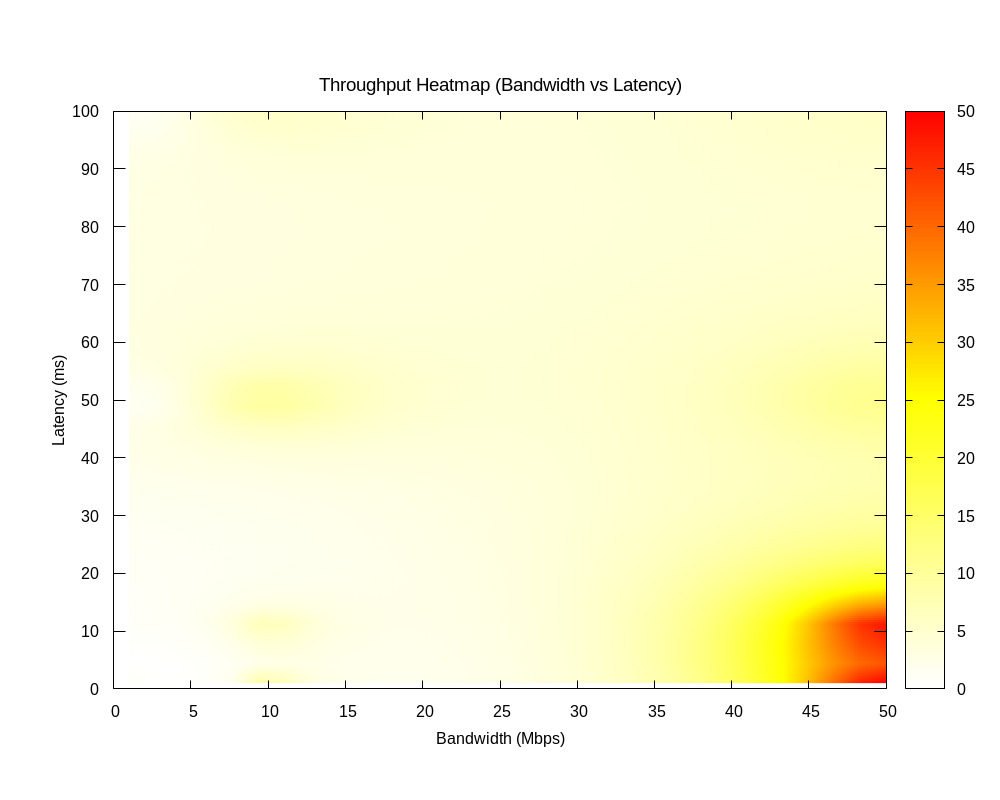
\includegraphics[width=1\columnwidth]{images/bandwidth-latenct.jpg}
    \end{center}
    \begin{itemize}
        \item The plot visualizes the relationship between bandwidth (x-axis) and latency (y-axis), and their impact on throughput.
        \item The heatmap shows that higher bandwidth and lower latency result in higher throughput, represented by the brighter yellow-to-red regions.
        \item The plot reveals an optimal bandwidth-latency sweet spot around 30-35 Mbps and 10-15 ms latency, where throughput is maximized.
        \item As bandwidth increases or latency worsens, the throughput gradually decreases, represented by the transition to cooler colors.
        \item The heatmap provides a clear visual representation of the interdependence between network parameters and their impact on overall system performance.
    \end{itemize}
\end{tcolorbox}

\questiontext{Q5. Explain in short what is the effect of changing the default MTU size.}

For this section, I will explain the effect of changing the default Maximum Transmission Unit (MTU) size on network performance.
First, Again creating two files named mtu.cc and mtu-bash.sh , first file for running the simulation and second file for automating the process.\\

\begin{tcolorbox}[colframe=blue!70!black, colback=blue!5!white, boxrule=0.4pt, width=\textwidth, sharp corners]
Main section of mtu.cc file is:-
\begin{center}
    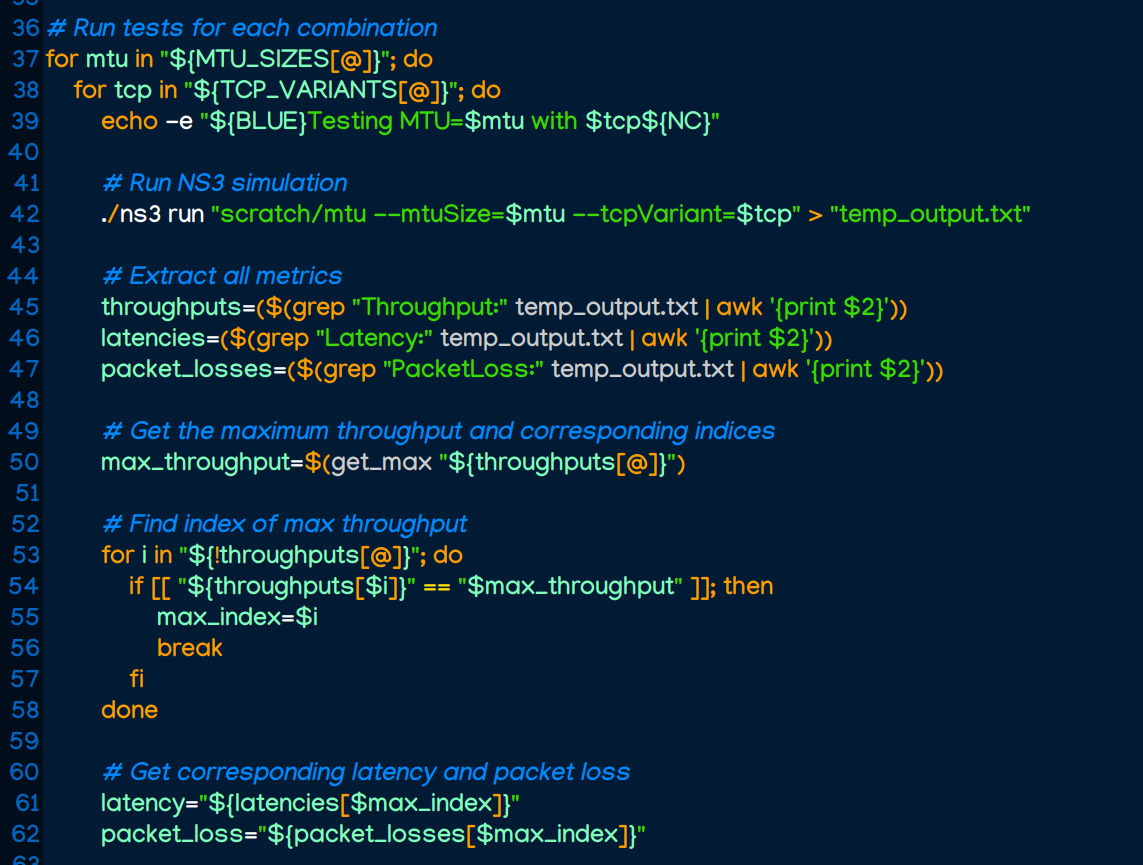
\includegraphics[width=1\columnwidth]{images/mtu-sim.jpg}
\end{center}
    \item \textbf{Image 1: Network Throughput, Latency, and Packet Loss Data}
    \begin{itemize}
    \item This image appears to be a text file containing numerical data related to network throughput, latency, and packet loss.
    \item The data is organized into sections, each with a header indicating the type of data it contains, such as \texttt{# MTU Throughput Latency PacketLoss}.
    \item The data is presented in a tabular format, with columns for different network parameters such as MTU (Maximum Transmission Unit), throughput, latency, and packet loss.
    \item The values in the data seem to be changing across different rows, suggesting that this is a set of test results or measurements taken over time or under different conditions.
    \end{itemize}
\end{tcolorbox}

\begin{tcolorbox}[colframe=blue!80!black, colback=blue!5!white, boxrule=0.4pt, width=\textwidth, sharp corners]
\begin{center}
    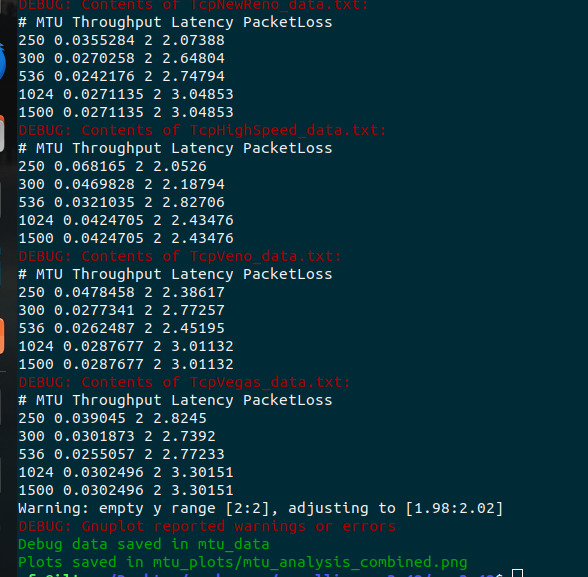
\includegraphics[width=1\columnwidth]{images/mtu-res.jpg}
\end{center}
\item \textbf{Image 2: Script for Analyzing Network Data}
\begin{itemize}
\item This image appears to be a script or code snippet written in a programming language, likely related to the analysis or processing of the network data shown in Image 1.
\item The script includes various commands and function calls, such as \texttt{Run tests for each combination}, \texttt{Extract all metrics}, and \texttt{Get the maximum throughput and corresponding indices}.
\item These commands suggest that the script is designed to perform analysis and data processing tasks on the network data, such as running simulations, extracting relevant metrics, and finding the maximum throughput and corresponding indices.
\item The script also includes some variable assignments and conditional statements, indicating that it is a more complex program that likely performs advanced data analysis and processing on the network data.
\end{itemize}

\end{tcolorbox}

\begin{tcolorbox}[colback=purple!5!white, colframe=purple!75!black, fonttitle=\bfseries, title=Question-2partA-4]
    Q6. Plot the rtt vs time graph and explain your inferences and observations.
\end{tcolorbox}

\begin{figure}[h]
    \centering
    \begin{minipage}{0.48\textwidth}
    \centering
    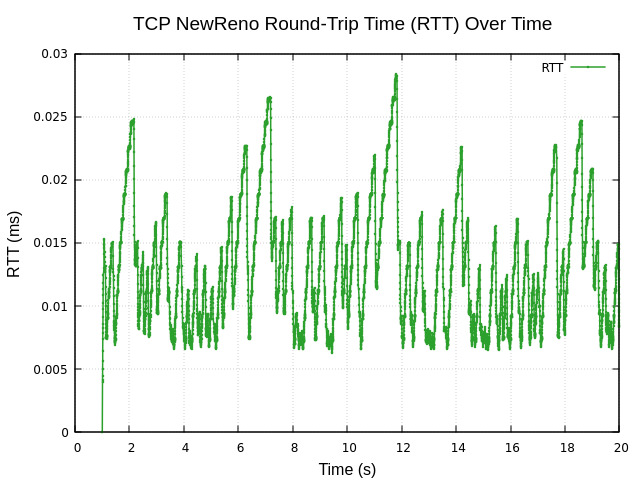
\includegraphics[width=\textwidth]{images/newreno_rtt.jpg}
    \subcaption{NewReno}
    \end{minipage}\hfill
    \begin{minipage}{0.48\textwidth}
    \centering
    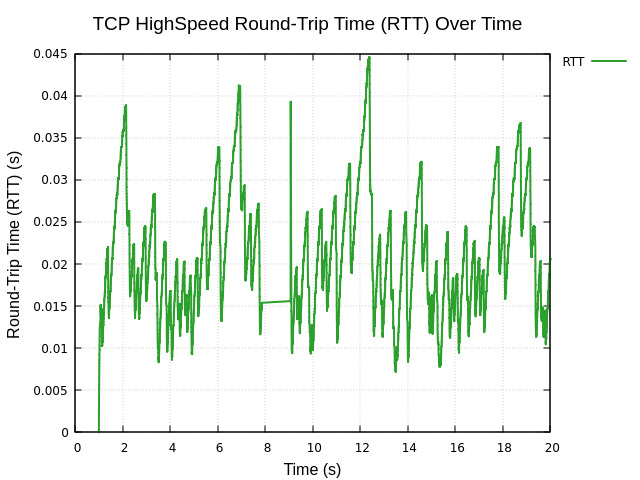
\includegraphics[width=\textwidth]{images/hs-rtt.jpg}
    \subcaption{HighSpeed}
    \end{minipage}
    \vspace{1em}
    
    \begin{minipage}{0.48\textwidth}
        \centering
        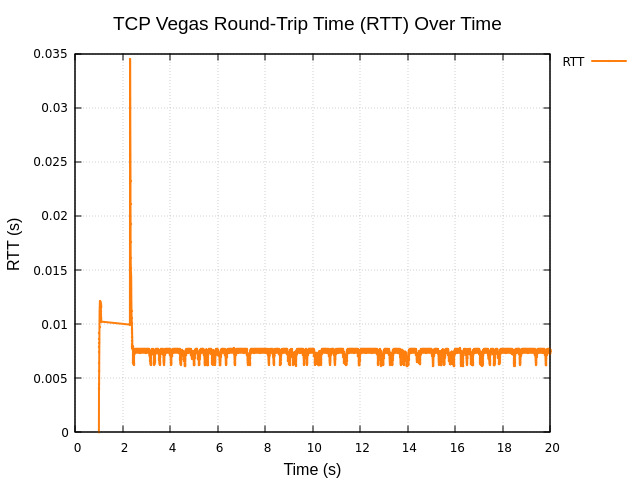
\includegraphics[width=\textwidth]{images/vegas_rtt.jpg}
        \subcaption{Vegas}
    \end{minipage}\hfill
    \begin{minipage}{0.48\textwidth}
        \centering
        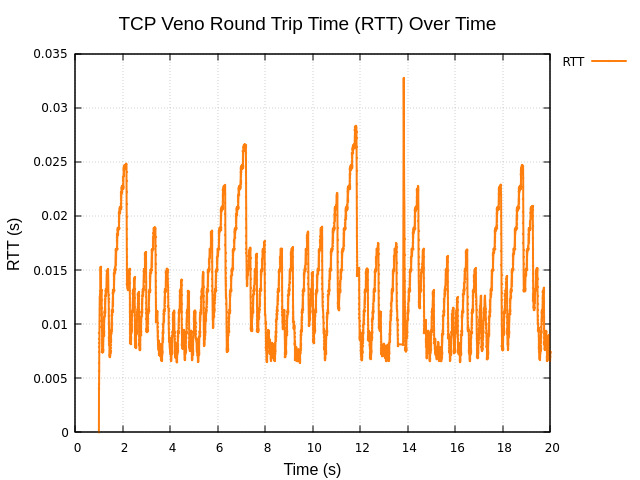
\includegraphics[width=\textwidth]{images/veno_rtt.jpg}
        \subcaption{Veno}
    \end{minipage}
    
    \caption{Round-Trip Time (RTT) vs. Time for Different TCP Variants}
    \label{fig:rtt_plots}
    \end{figure}
    \subsection{NewReno}
    \textbf{Inference:} The RTT graph for NewReno shows significant fluctuations, with sharp peaks and valleys. This indicates an aggressive and reactive congestion control mechanism.\\
    \textbf{Observation:} The large RTT variations suggest NewReno is unsuitable for networks with high bandwidth-delay products, struggling to maintain stable throughput.
    
    \subsection{HighSpeed}
    \textbf{Inference:} The RTT graph for HighSpeed displays a smoother, more controlled pattern than NewReno, indicating a more adaptive congestion control algorithm.\\
    \textbf{Observation:} This stability aligns with HighSpeed's design for high-speed networks, where sophisticated window adjustments help maintain consistent performance.
    
    \subsection{Vegas}
    \textbf{Inference:} Vegas exhibits a stable RTT throughout the observation, with few spikes, reflecting its proactive congestion avoidance.\\
    \textbf{Observation:} The smooth RTT pattern indicates Vegas's effectiveness in maintaining performance through RTT-based congestion control, adjusting the window to avoid fluctuations.
    
    \subsection{Veno}
    \textbf{Inference:} Veno's RTT plot shows smooth segments interspersed with spikes, suggesting a balanced congestion control approach.\\
    \textbf{Observation:} Veno effectively differentiates congestion-related losses from random losses, leading to a balanced RTT pattern, suitable for mixed wired and wireless networks.


\section{PART-B}
\begin{verbatim}
a. You need to create a new CCA named Tcp<first_name> and you need to try 
to improve TcpNewReno’s performance. 

b. You need to focus only on the SlowStart phase and in order to improve it 
you need to replace Reno’s slow start with TCP Hystart (whose implementation
can be found in src/internet/model/tcp-cubic.cc which is ns-3’s Tcp Cubic 
implementation).

c. You aim and try to make the slow start phase more intelligent with better 
exit points by doing this (more about Hystart at Reference a) but once you 
have done this you need to evaluate your algorithm’s performance, so consider
the dumbbell topology in demo.cc, make all the flows TCP and evaluate the 
standard metrics like throughput, congestion window, ssthresh, rtt variation 
qbetween your algo and NewReno.
\end{verbatim}

\large{\textbf{Solution:}}\\
For this part, I will create a new congestion control algorithm named TcpAyush, focusing on improving the Slow Start phase by replacing Reno's slow start with TCP Hystart.\\
All the class and variables are defined in the tcp-ayush.h and functions in tcp-ayush.cc files.\\
Following are the main sections of the code in tcpayush.h :-
\begin{center}
    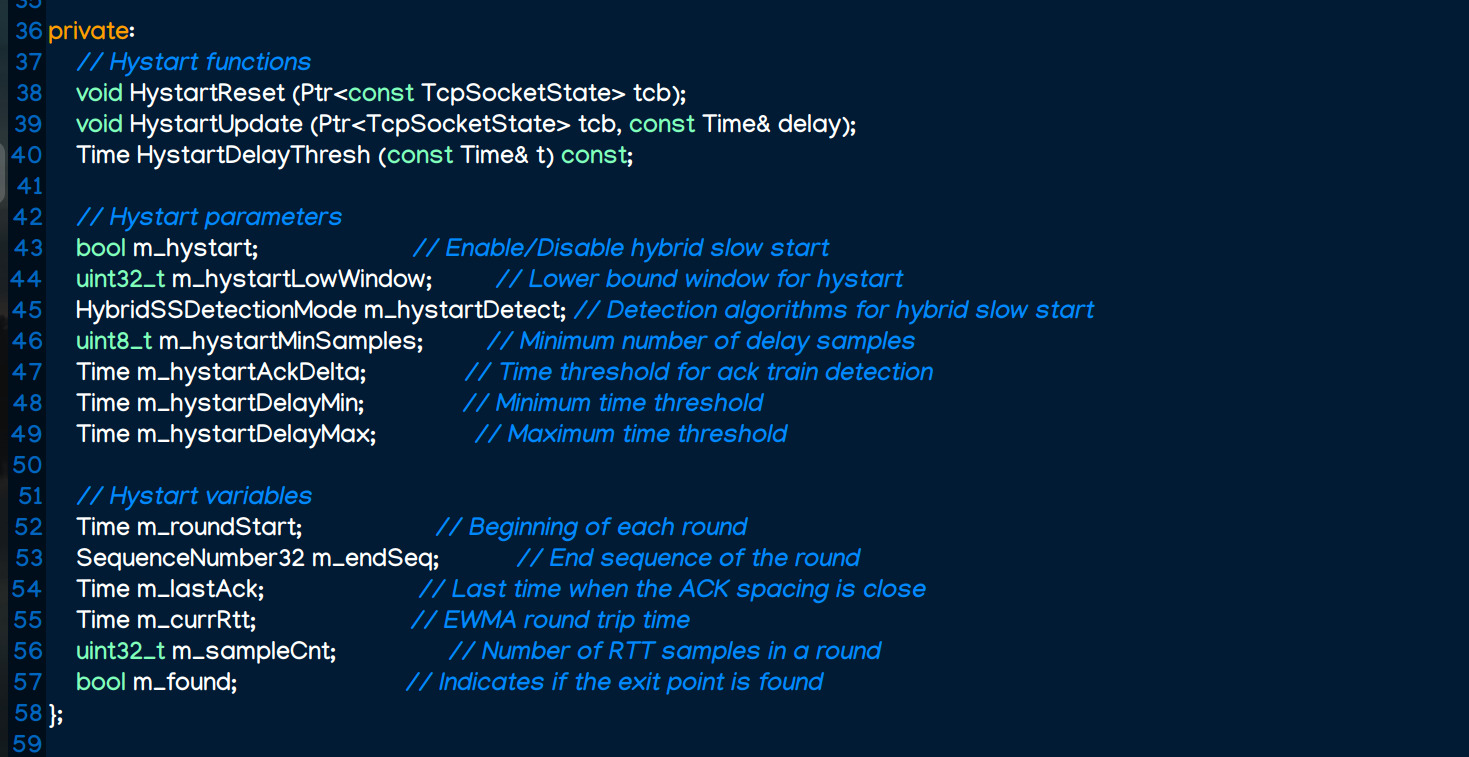
\includegraphics[width=1\columnwidth]{images/tcpayush.h.jpg}
\end{center}
\begin{center}
    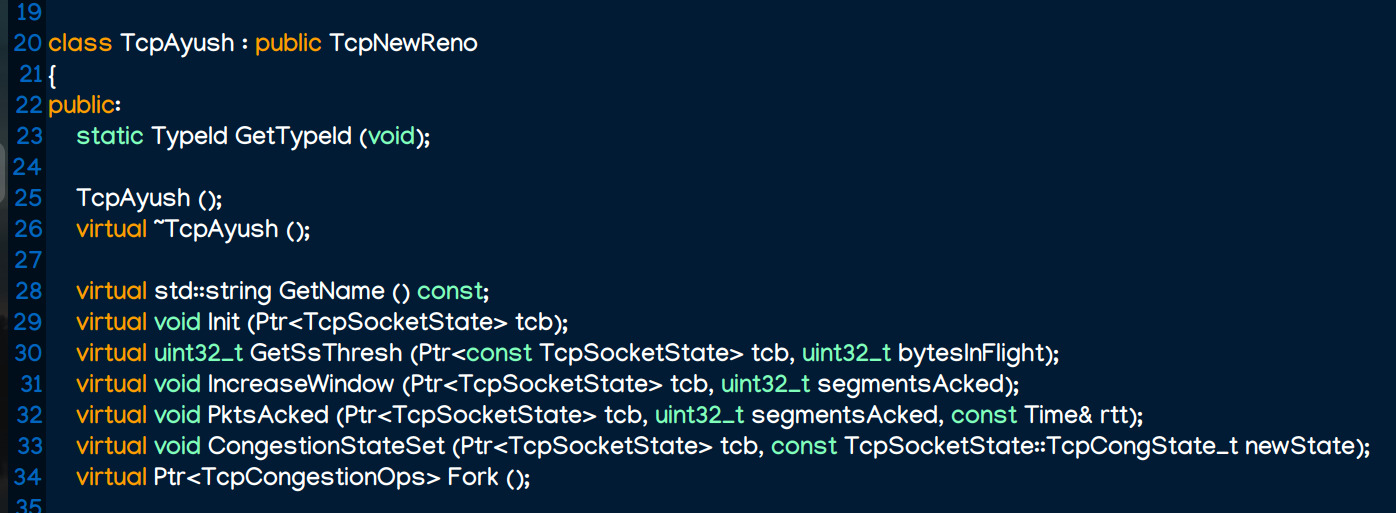
\includegraphics[width=1\columnwidth]{images/tcpayush-functions.jpg}
\end{center}
In this project, I improved the \texttt{TcpAyush} congestion control algorithm by referencing the \textcolor{blue}{TCP Cubic} implementation in \texttt{ns-3}, particularly integrating \textcolor{teal}{Hystart's} intelligent slow-start mechanism. The focus was on making the slow-start phase more adaptive by incorporating \textcolor{purple}{dynamic exit points}, as recommended in the reference material.

The primary enhancements included:
\begin{itemize}
    \item Adding Hystart-inspired \textcolor{red}{adaptive exit criteria} for the slow-start phase.
    \item Adjusting \textcolor{purple}{thresholds} within the slow-start mechanism to better respond to \textcolor{orange}{real-time network conditions}.
\end{itemize}

To evaluate performance, I tested \texttt{TcpAyush} using the \textcolor{blue}{dumbbell topology} in \texttt{demo.cc}, which allows for a clear comparison of \textcolor{teal}{throughput results}. Several modifications were necessary in \texttt{demo.cc} to properly accommodate and benchmark \texttt{TcpAyush}, ensuring reliable and meaningful performance metrics.

With these adjustments in place, the next step will involve running \textcolor{purple}{simulations} to analyze the throughput results.

\begin{center}
    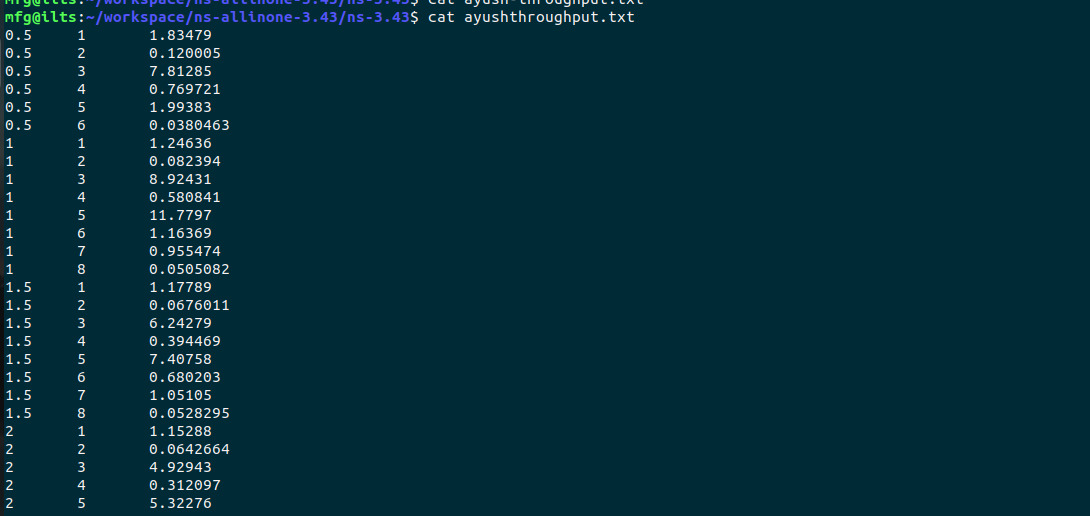
\includegraphics[width=1\columnwidth]{images/ayush-t.jpg}
    \caption{Throughput file for tcpayush}
\end{center}

\begin{center}
    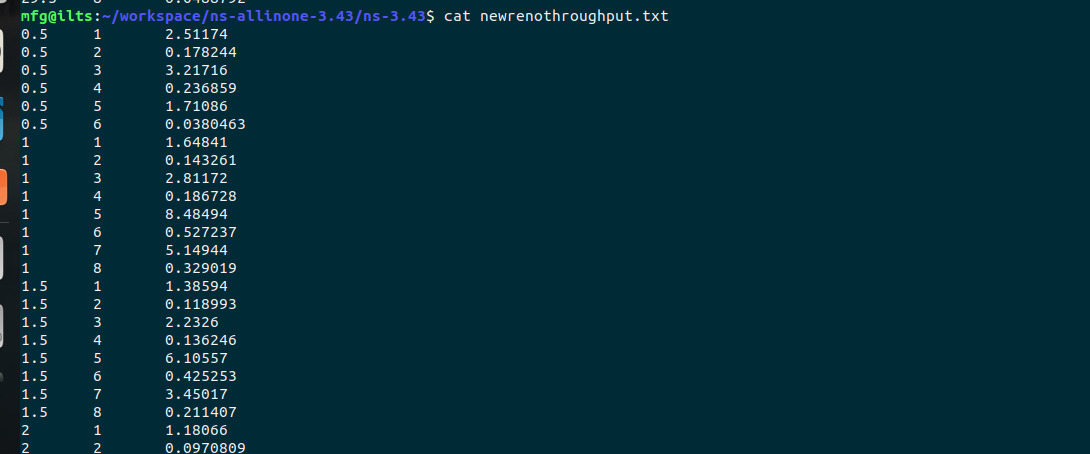
\includegraphics[width=1\columnwidth]{images/newreno-t.jpg}
    \caption{Throughput file for TcpNewReno}
\end{center}

\begin{verbatim}
d. Also, calculate the value of Jain’s fairness index (more 
about this at Reference b) by varying the number of flows
as 4,8,16,20. So in the first run of your experiment all 
the flows will be using TcpNewReno so that becomes your 
baseline readings for comparison and in the second run of 
experiment, half of the flows will be using TcpNewReno while
the other half of the flows will be using your new CCA. 
Create a table like shown below and populate it with the 
fairness values achieved in each case.
\end{verbatim}

For this, I created a bash file \texttt{\textcolor{blue}{jain-index.sh}} to calculate the \textcolor{teal}{Jain's fairness index} by varying the \textcolor{purple}{number of flows} and comparing the performance of \texttt{\textcolor{blue}{TcpNewReno}} with \texttt{\textcolor{blue}{TcpAyush}}. 

There are two main tasks: first, to create \textcolor{orange}{4 files} for mixed flows, and then \textcolor{orange}{4} for NewReno flows. For this task, I created \texttt{\textcolor{blue}{create-file.sh}} to automate the process of generating files for both \textcolor{teal}{mixed} and \textcolor{teal}{NewReno} flows.

This looks like:

\begin{center}
    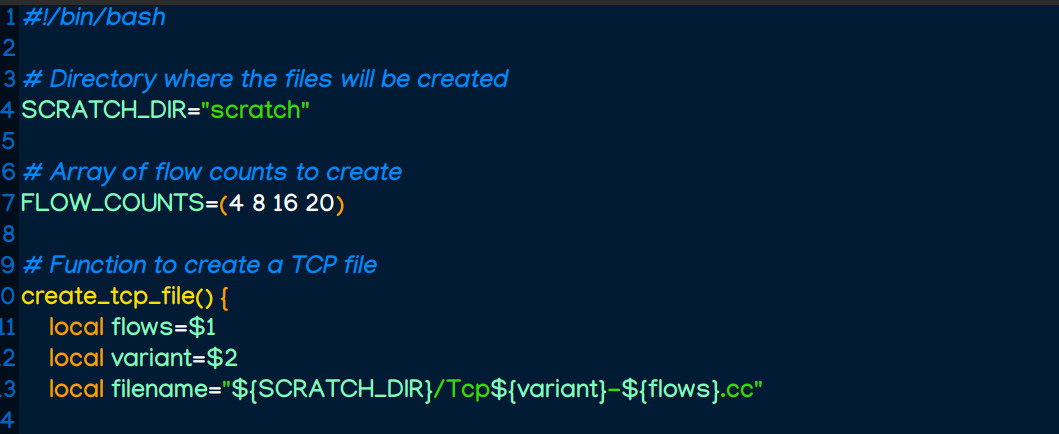
\includegraphics[width=1\columnwidth]{images/create-sh.jpg}
    \caption{Code to create file and save it in scratch directory}
\end{center}

\begin{center}
    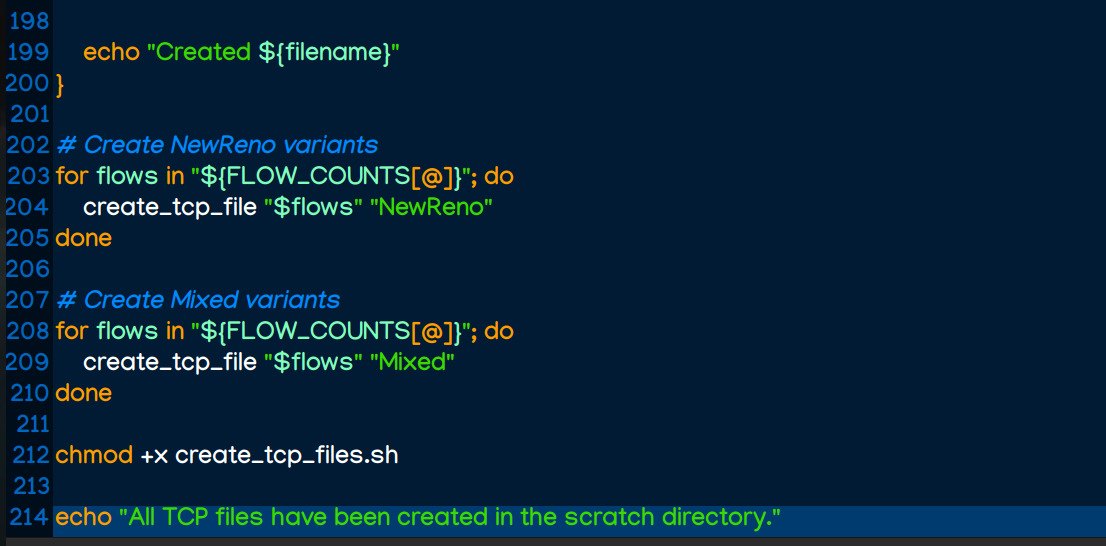
\includegraphics[width=1\columnwidth]{images/create-sh2.jpg}
    \caption{Taking input for flows and creating new file with this flow value.}
\end{center}

Second task is to calculate the Jain's fairness index for each case and populate the table \\
with the fairness values achieved in each case.\\

\begin{center}
    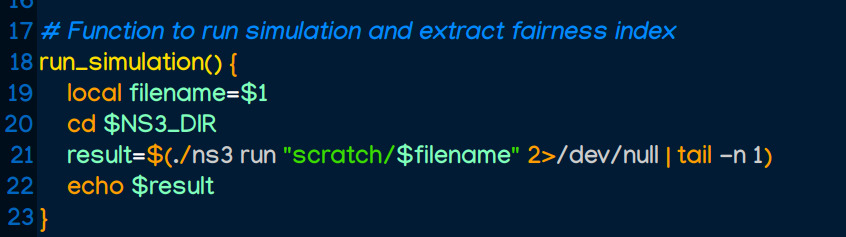
\includegraphics[width=1\columnwidth]{images/jain-sim.jpg}
    \caption{Simulation code to calculate jain\_index function}
\end{center}

\begin{center}
    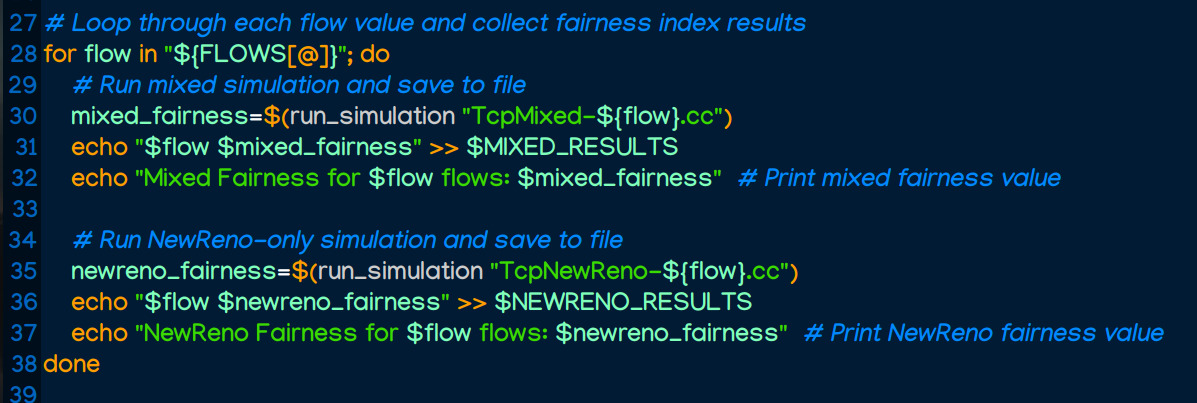
\includegraphics[width=1\columnwidth]{images/jain-sim2.jpg}
    \caption{Main code to run calculate jain\_index function and save it in file}
\end{center}

Result of \textcolor{orange}{Above code} is:-
\begin{center}
    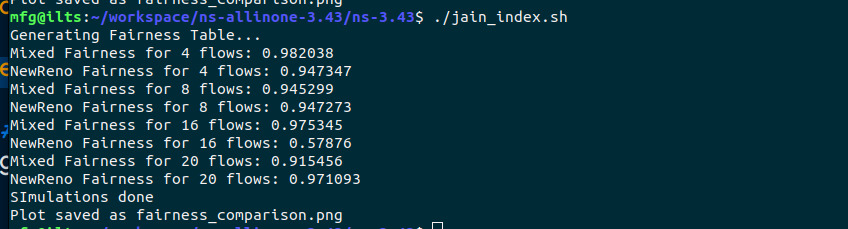
\includegraphics[width=1\columnwidth]{images/bash-jain.jpg}
    \caption{Jain's Fairness Index for Different Number of Flows}
\end{center}
\begin{center}
    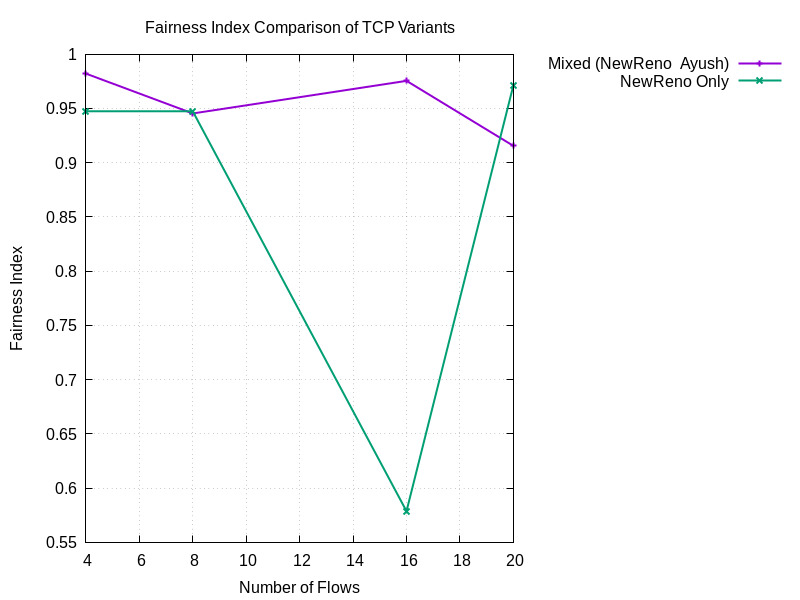
\includegraphics[width=1\columnwidth]{images/jain-res.jpg}
    \caption{Plot of jain index value for tcpayush and tcpnewreno}
\end{center}

\begin{verbatim}
e. Plot the necessary graphs for all the metrics (throughput, congestion window, ssthresh,
rtt) collected.
\end{verbatim}
All the plots are as follows:
1) RTT Comparison for TcpAyush and TcpNewReno
\begin{center}
    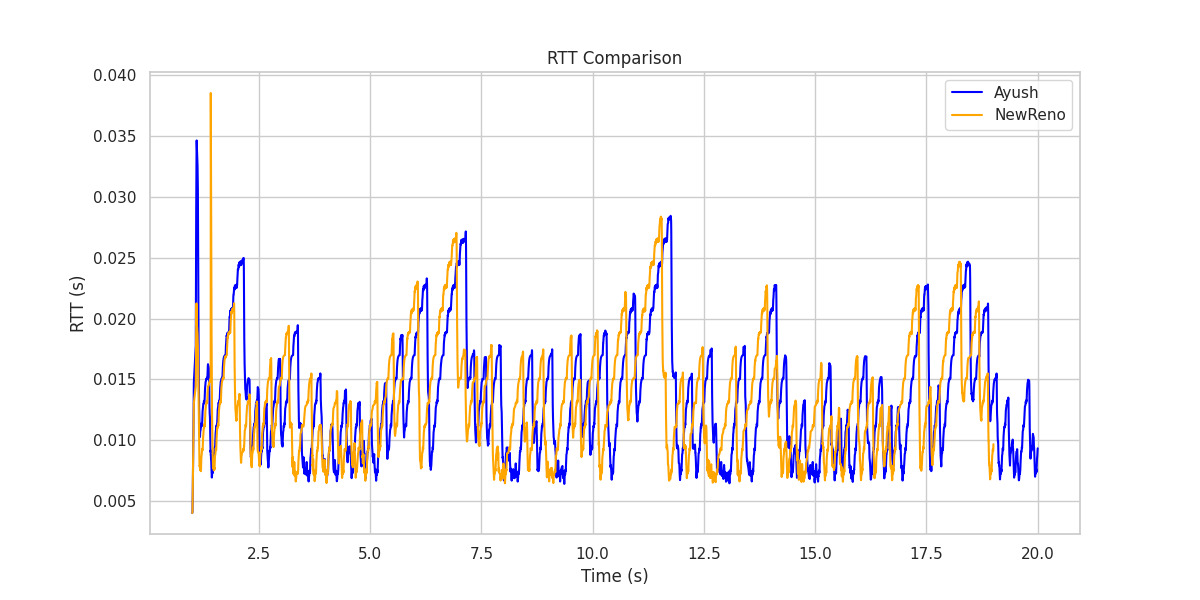
\includegraphics[width=1\columnwidth]{images/rtt-comp.jpg}
\end{center}
2) Congestion Window Comparison for TcpAyush and TcpNewReno
\begin{center}
    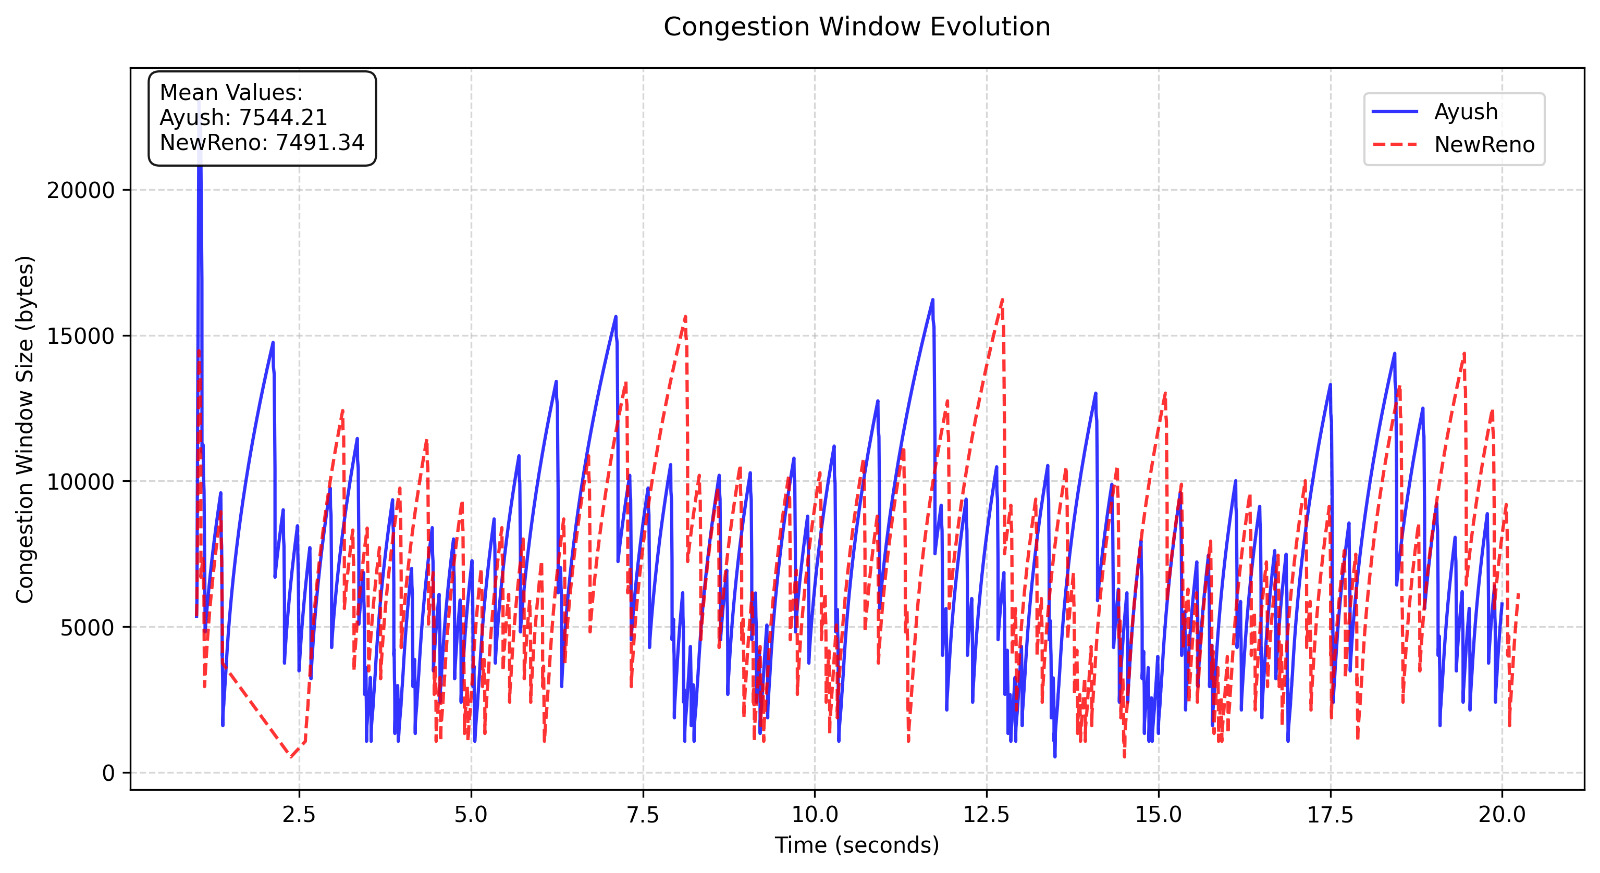
\includegraphics[width=1\columnwidth]{images/cwnd-comp.jpg}
\end{center}
3) Throughput Comparison for TcpAyush and TcpNewReno
\begin{center}
    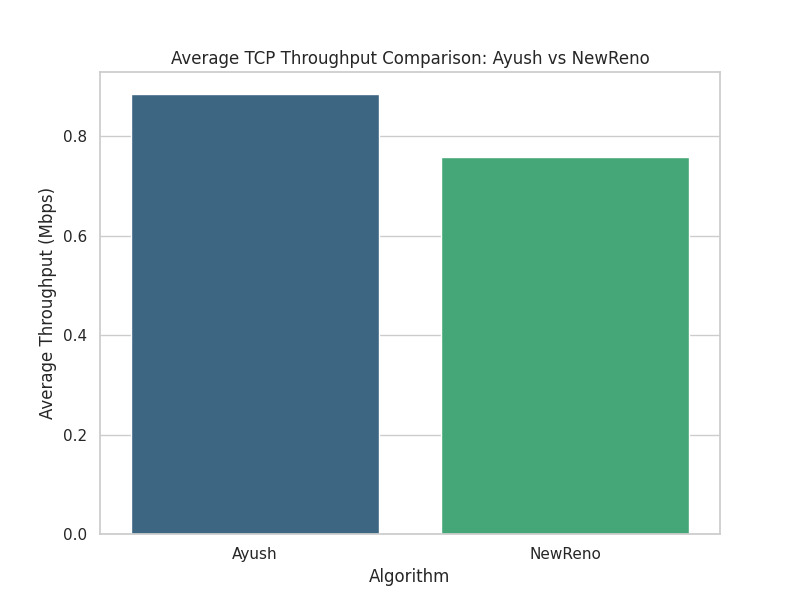
\includegraphics[width=1\columnwidth]{images/t-comp.jpg}
\end{center}
4) SSThresh Comparison for TcpAyush and TcpNewReno
\begin{center}
    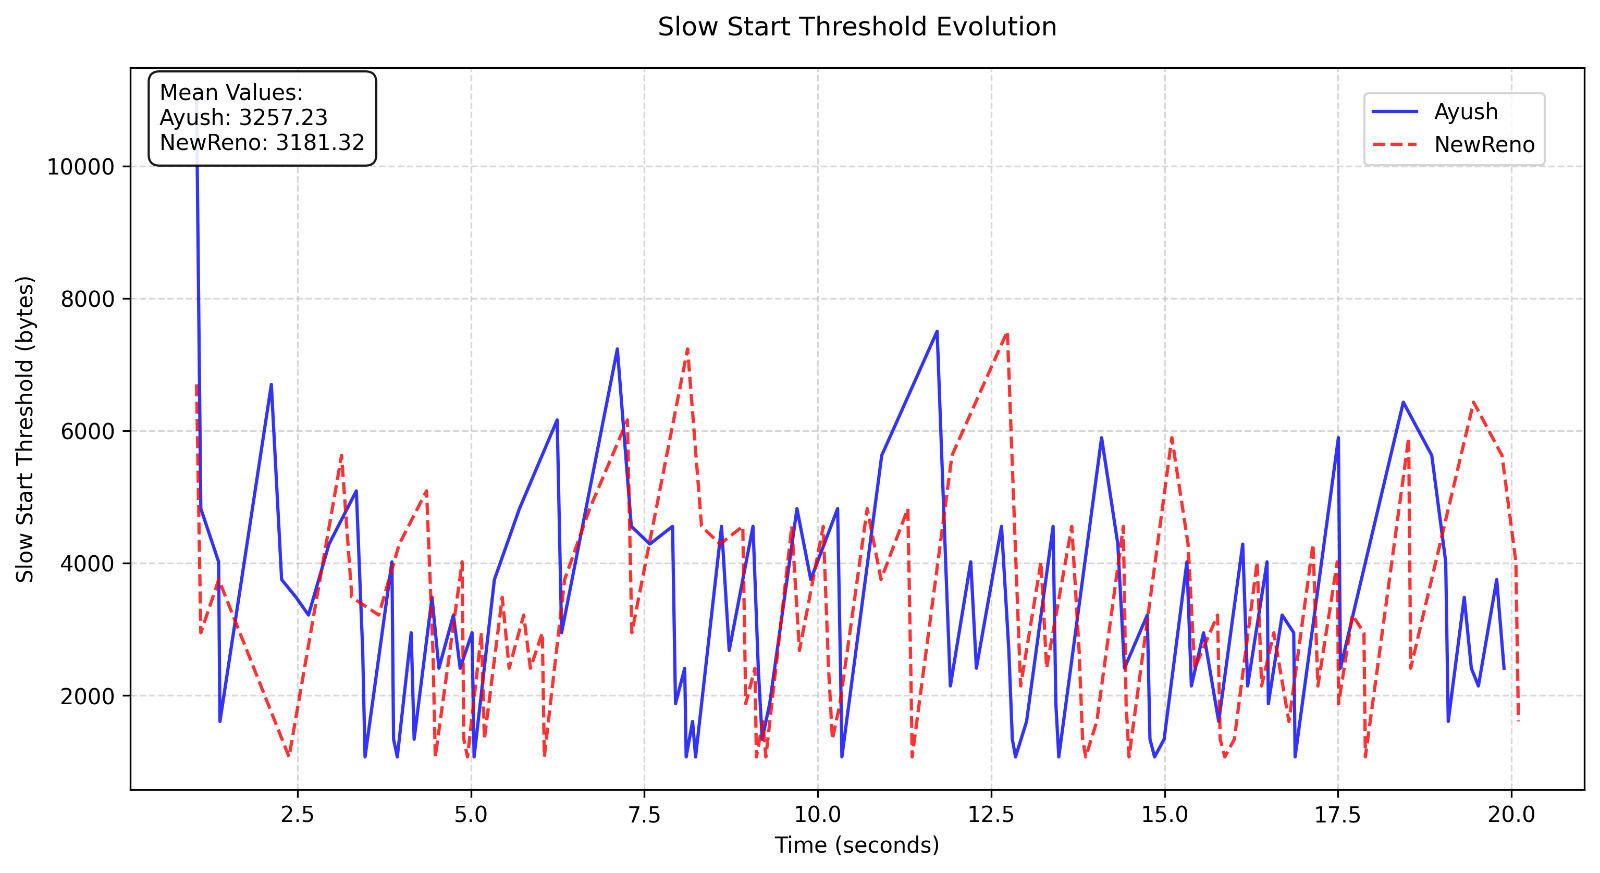
\includegraphics[width=1\columnwidth]{images/ss-comp.jpg}
\end{center}

\begin{verbatim}
f. Finally, try to justify and explain the results of the comparison thus obtained.
\end{verbatim}

\textbf{\textcolor{teal}{RTT (Round Trip Time) Comparison:}}

\begin{itemize}
    \item Both algorithms show similar \textcolor{purple}{RTT} patterns over time, with values fluctuating between approximately \textcolor{orange}{0.005} and \textcolor{orange}{0.035 seconds}.
    \item The \textcolor{purple}{RTT} fluctuations are highly correlated between both algorithms.
    \item Neither algorithm consistently maintains a lower \textcolor{purple}{RTT} than the other, suggesting \textcolor{teal}{similar delay characteristics}.
\end{itemize}

\textbf{\textcolor{teal}{Average TCP Throughput:}}

\begin{itemize}
    \item \texttt{Ayush} achieves slightly higher throughput (\textcolor{purple}{0.85 Mbps}) compared to \texttt{NewReno} (\textcolor{purple}{0.75 Mbps}).
    \item This represents approximately a \textcolor{teal}{13\% throughput improvement} with \texttt{Ayush}.
    \item The higher throughput may indicate more efficient \textcolor{purple}{bandwidth utilization} by \texttt{Ayush}.
\end{itemize}

\textbf{\textcolor{teal}{Slow Start Threshold Evolution:}}

\begin{itemize}
    \item Mean values: \texttt{Ayush} (\textcolor{purple}{3257.23 bytes}) vs \texttt{NewReno} (\textcolor{purple}{3181.32 bytes}).
    \item Both algorithms exhibit similar patterns of \textcolor{teal}{threshold adjustments}.
    \item \texttt{Ayush} maintains a slightly higher average threshold, allowing more \textcolor{purple}{aggressive sending behavior}.
    \item This higher threshold in \texttt{Ayush} may explain its \textcolor{teal}{better throughput}.
\end{itemize}

\textbf{\textcolor{teal}{Congestion Window Evolution:}}

\begin{itemize}
    \item Mean values: \texttt{Ayush} (\textcolor{purple}{7544.21 bytes}) vs \texttt{NewReno} (\textcolor{purple}{7491.34 bytes}).
    \item Both algorithms display similar patterns in \textcolor{teal}{window size adjustments}.
    \item \texttt{Ayush} maintains a marginally larger average window size.
    \item The window size variations in \texttt{Ayush} are more pronounced, suggesting \textcolor{purple}{more dynamic adjustments} to network conditions.
\end{itemize}

\textbf{\textcolor{teal}{Justification of Results:}}

\textbf{Improved Performance:}
\begin{itemize}
    \item \texttt{Ayush}'s improved throughput can be attributed to its slightly higher average \textcolor{teal}{congestion window} and \textcolor{teal}{slow-start threshold}.
    \item The algorithm appears to be more aggressive in \textcolor{purple}{utilizing available bandwidth} while maintaining similar \textcolor{purple}{RTT characteristics}.
\end{itemize}

\textbf{Stability:}
\begin{itemize}
    \item Despite its more aggressive behavior, \texttt{Ayush} maintains \textcolor{purple}{RTT values} comparable to \texttt{NewReno}.
    \item This suggests that the improved throughput does not lead to increased \textcolor{purple}{network congestion}.
\end{itemize}

\textbf{Adaptability:}
\begin{itemize}
    \item The more dynamic congestion window adjustments in \texttt{Ayush} indicate better \textcolor{teal}{responsiveness to network conditions}.
    \item This adaptability likely contributes to its ability to maintain higher throughput while keeping \textcolor{purple}{RTT} within a reasonable range.
\end{itemize}

\textbf{Trade-offs:}
\begin{itemize}
    \item The minor differences in mean values suggest that \texttt{Ayush} achieves subtle yet effective improvements over \texttt{NewReno}.
    \item The similar \textcolor{purple}{RTT patterns} indicate that the throughput gains do not compromise \textcolor{teal}{network stability}.
\end{itemize}



\end{document}
